\chapter{Introduction}
\label{sec:intro}
We live in an age of data. Sensors are deployed and images are taken anywhere we can get them in order to collect information about our environment. In particular, Neuroimaging data is now being collected in large volumes globally. With initiatives such as the 1000 Functional Connectome Project and the International Neuroimaging Data-Sharing Initiative \cite{fcpindi}, and the Human Connectome Project \cite{hcp}, accessibility to structural, functional, and diffusion weighting MRI data is greater than ever. Open-access repositories such as LONI's IDA\cite{loni1} and NITRC distribute this data and associated covariates to the community. Tools such as FSL \cite{fsl1,fsl2,fsl3}, ANTs \cite{ants}, DiPy \cite{dipy}, as well as many others, enable complex processing and quantitative analysis of this data to be performed with relative ease by scientists. With the advent of cloud computing resources such as Amazon Web Services' Elastic Cloud Computing (EC2) and the ever-expanding pool of available computational resources, all of this processing can be done quickly and cheaply, as well.

However, coincident with the availability of all of these tools, we have the encountered the problem that analysis of neuroimaging data is non-uniform. As a result, studies have shown that medical research is plagued by a lack of reproducibility \cite{reliability1,reliability2}. Data collection procedures in MRI are non-standardized and vary wildly in terms of image acquisition protocol, parameter selection, signal strength, as well as downstream factors such as data storage format on disk. As a result, it is extremely difficult to compare findings from one study with those collected as part of another. Current processing strategies involve tuning parameters, and over-fitting them to a dataset, rather than applying more general methods which have been shown to work globally. However, processing all publicly available data uniformly is non-trivial, as existing end-to-end processing pipelines such as CPAC \cite{cpac}, PANDA \cite{panda}, CMTK \cite{cmtk}, MIGRAINE \cite{migraine}, and MRCAP \cite{mrcap}, have been designed with complex setup routines and are limited in their ability to run in parallel and scalable cluster-based computing fashion. Furthermore, packaging such a tool in an accessible interface such as a web service has yet to be done, and requires different domain knowledge often uncommon in the neuroscience community. Such a service would serve as an interface, further lowering the barrier to entry for scalable connectome estimation and analysis. Lastly, very few publicly available connectomes exist, and those that do have been processed inconsistently and therefore cannot be effectively compared to one another.

Leveraging existing research tools in the marketplace, we have built an open-source end-to-end structural connectome estimation pipeline from diffusion weighted MR images, entitled NeuroData's MRI to graphs pipeline (ndmg). The pipeline has been developed with a core set of parameters which have been chosen to optimize the downstream inference of graphs in a principled manner. A web service has been deployed, in which users can upload raw image data and receive a processed connectome at no cost. All known publicly sharable diffusion and structural MRI datasets have been processed using ndmg and over $100,000$ graphs across multiple scales have been made publicly available for analysis. Finally, we illustrate the significance of batch effects in data collection, and make efforts to mitigate them.

There now exists open source code that anyone can download and install on their local computer to estimate connectomes quickly and reliably. A public facing database of uniformly estimated connectomes enables exploratory analysis about the structure of the brain. Here we will discuss the principles underlying and techniques used in creating ndmg, and introduce the largest known publicly available connectome database to date.
%=========================
%%% End Introduction

\chapter{Background}
\label{sec:bg}
\section{What is a Connectome?}
\label{sec:define}
As defined in 2005 by Olaf Sporns, a connectome is "a comprehensive structural description of the network of elements and connections forming the brain" \cite{Sporns2005}. As different problems find different scales of data useful, multiple definitions of connectomes have been given across multiple scales and resolutions. These definitions range in scale from sub-cellular resolution images of the brain, in which a connectome consists of neurons as nodes in a graph with the synapses and gap junctions between them as edges, up to several cubic $mm$ brain regions as nodes where edges are defined as white matter pathways between. The highest resolution connectome we describe is referred to as a \textit{micro-} or \textit{nanoscale} connectome. Current techniques that exist for acquiring data at this resolution (on the range of nanometers) are often performed with electron microscopy. This requires post mortem tissue, and resulting images are difficult to deal with as they take up many terabytes of space on disk for even small (cubic millimeter) cortical areas.

At the level of the \textit{macroscale} connectome, we are able to quickly acquire a coarse map of the entire brain in a live human subject. Using Magnetic Resonance Imaging (MRI), we are able to get these images non-invasively at a millimeter resolution, and are able to image the same tissue multiple times with different contrasts. For the sake of this document, when referring to a connectome we will henceforth be referring specifically to a macroscale connectome.

To summarize the above, we can think of the brain as a map. At the finest level, we see driveways, side-streets, cars, houses, and shops, representing all of our cells and processes. As we zoom out, the finer details begin to fade, but we start seeing a more comprehensive view of neighborhoods, communities, and a city. As we continue to pan higher we lose all sense of small communities, but gain a sense of cities, provinces, states, and even countries, as well as the pathways - or roads - connecting them. What we aim to do in MR connectomics is drop pins in cities on our map (nodes), and trace the roads between them with pieces of string (edges).

\section{Acquiring Data For Connectomics}
\label{sec:acquire}
MRI is an extremely popular form of imaging in modern medicine. It is a non-invasive technique which relies on the manipulation of nuclear spin of atoms - mostly Hydrogen - within the sample volume in order to produce contrast. Nishimura \cite{nishimura} provides a detailed overview of how MRI works, including development of different sequences for obtaining different forms of contrast in the images, and is recommended if you wish to explore MRI itself in further detail.

The brain consists of two major forms of tissue: gray matter and white matter. Gray matter contains a high density of cell bodies (i.e. neurons), and represents processing in the brain. White matter, in contrast, contains a high density of connective tissue (i.e. myelinated axons) and can be thought of representing gross scale communication between brain regions. As these two types of tissue are significantly different in their structure, they also exhibit different properties which can be detected by an MRI scanner.

There are near infinite types of MRI sequences that could exploit these differences in brain tissue, though those perhaps most notable are functional MRI (fMRI), structural T1 MRI (MPRAGE), and diffusion weighted MRI (DWI), which includes techniques such as Diffusion Tensor Imaging (DTI), Diffusion Spectrum Imaging (DSI), and High Angular Resolution Diffusion Imaging (HARDI). Each of these images are defined for the type of contrast they provide. In the case of fMRI, high intensity in a voxel (3-dimensional pixels) indicates high amounts of blood flow passing through that region. MPRAGE scans have contrast based on T1 (longitudinal) relaxation of tissue, and provide the clearest/highest quality images of whole brain structure of those that we discuss here. These scans most closely resemble what our brain looks like, and are important when comparing results across subjects. Finally, DTI images are 4-dimensional images ($x \times y \times x \times D$, where D is the number of diffusion directions) that indicate the directional rates of water diffusion along an axis as defined by the diffusion direction of the scan. Inherent in the structure of the brain, the primary direction of diffusion of water is highly correlated to the principal axis of a myelinated axon, thus, these images consist primarily of white matter pathways.


\begin{figure}[h!]
\centering
\begin{subfigure}[h!]{0.45\textwidth}
\centering
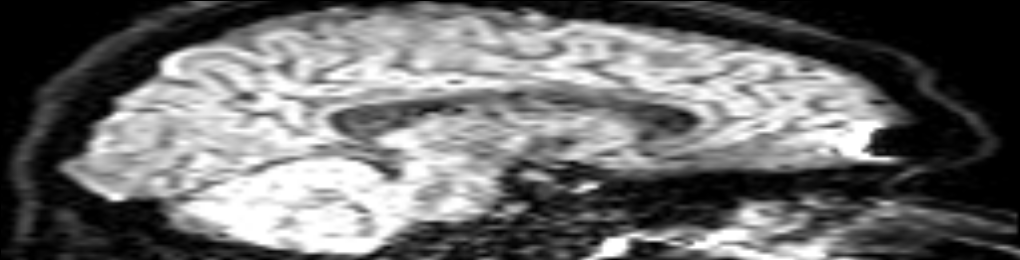
\includegraphics[scale=0.2]{./figs/KKI2009-01-DTI.png}
\makeatletter
\let\@currsize\normalsize
\caption{Single DTI volume}
\end{subfigure}
\begin{subfigure}[h!]{0.45\textwidth}
\centering
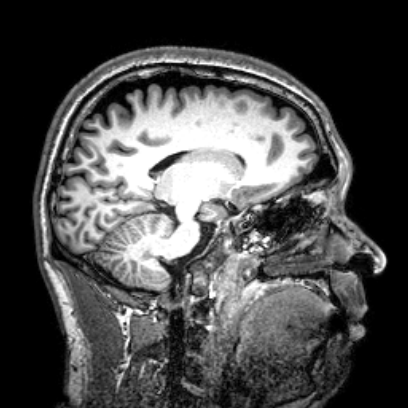
\includegraphics[scale=0.35]{./figs/KKI2009-01-MPRAGE.png}
\makeatletter
\let\@currsize\normalsize
\caption{MPRAGE volume}
\end{subfigure}
\makeatletter
\let\@currsize\normalsize
\caption{Structural MRI image volumes. Note that the DTI volume is anisotropic (lower resolution in one direction), thus without warping appears compressed.}
\label{fig:mri}
\end{figure}


This thesis is not concerned with the acquisition of MR images, nor it is concerned with functional imaging methods. Though much imaging data is obtained in practice, it is tragically under used in quantitative analysis; here, I provide an approach for numerically analyzing and summarizing images of the brain in a fashion which opens the door for exploration of structural network biomarker development in the human brain. If we again consider our map, fMRI represents masses of cars on the road, MPRAGE the cities, and DTI the highways themselves. Here, when estimating a structural connectome, we can ignore the cars (fMRI) and focus on our cities and roadways (i.e. MPRAGE and DTI scans). Figure \ref{fig:mri} shows both diffusion and structural MR images.

\section{Building A Connectome}
\label{sec:previous}
The notion of creating an MR connectome is not a new one - along with the initial definition of connectomes in 2005 by Sporns, Hagmann explored this idea in his PhD thesis entitled \textit{From diffusion MRI to brain connectomics} \cite{hagman2005}. Many processing tools have since been developed or improved for processing MR images including FSL \cite{fsl1, fsl2,fsl3}, ANTs \cite{ants}, Camino \cite{camino}, JIST \cite{jist}, DiPy \cite{dipy}, and others. Each of these tools performs some subset of transformations to MR data such as denoising, image registration, tensor or orientation distribution function (ODF) estimation, and deterministic or probabilistic tractography. Several efforts have also existed to pipeline these tools together into a single tool, including MR-CAP \cite{mrcap}, MIGRAINE \cite{migraine}, Panda \cite{panda}, and CMTK \cite{cmtk}, to name a few. These efforts have been greatly successful, and for the first time enabled the community to produce maps of the brain at a millimeter resolution. However, these solutions are not without their limitations. Previous pipelines have been developed without accessibility as a primary concern, have had difficulty scaling to large datasets, and often relied on setup routines and dependencies that are relatively complex for a non-tech savvy user. They also have not been validated to produce results which are reliable across datasets or parameters. These pipelines have also relied on parameters which could be tuned by the user, resulting in widely varying connectomes produced which become incredibly difficult to compare. These limitations have made estimation of connectomes in bulk a difficult task, let alone downstream analysis upon them. Here is where we enter the scene, as we attempt to tackle these limitations and provide a reliable, consistent, simple, and scalable solution to structural connectome estimation from diffusion weighted MRI that is openly available for the community to both use and improve upon.

%%% Begin Methods
%=========================
\chapter{Methods}
\label{sec:ndmg}
We set out with the goal of developing a connectome estimation pipeline that maintained the strengths of previous pipelines, as well as providing a scalable, robust, and reliable solution to this difficult task. Expanding concepts deployed in our previous pipelines, MIGRAINE and MRCAP, we have provided an open-source Python package and pipeline, for which documentation and source code can be found at \url{http://m2g.io}. The ndmg pipeline through it's derivatives has been validated using a statistically principled approach, and services now exist which significantly lower the barrier for entry to both connectome generation and analysis.
\section{NeuroData's MRI Graphs}
\label{sec:ndmg-over}
We have produced an end-to-end one-click open-source pipeline, called NeuroData's MRI Graph pipeline (ndmg). A high level description of the ndmg pipeline can be seen in Figure \ref{fig:ndmg-simple}. The ndmg pipeline accepts subject specific DTI and MPRAGE scans; gradient direction and intensity parameter files associated with the DTI image; a template image; and, an atlas containing regions of interest (ROIs) in the brain.

The pipeline performs a series transformations on this data, which will be elaborated on shortly, and returns a graph in which the nodes are defined by ROIs in the atlas, and edges defined by inter-ROI connectivity. Exploiting existing tools such as FSL, Networkx, and DiPy, ndmg has been packaged in Python and can be run with a single command.

\begin{figure}[h!]
\centering
\begin{subfigure}[h!]{0.8\textwidth}
\centering
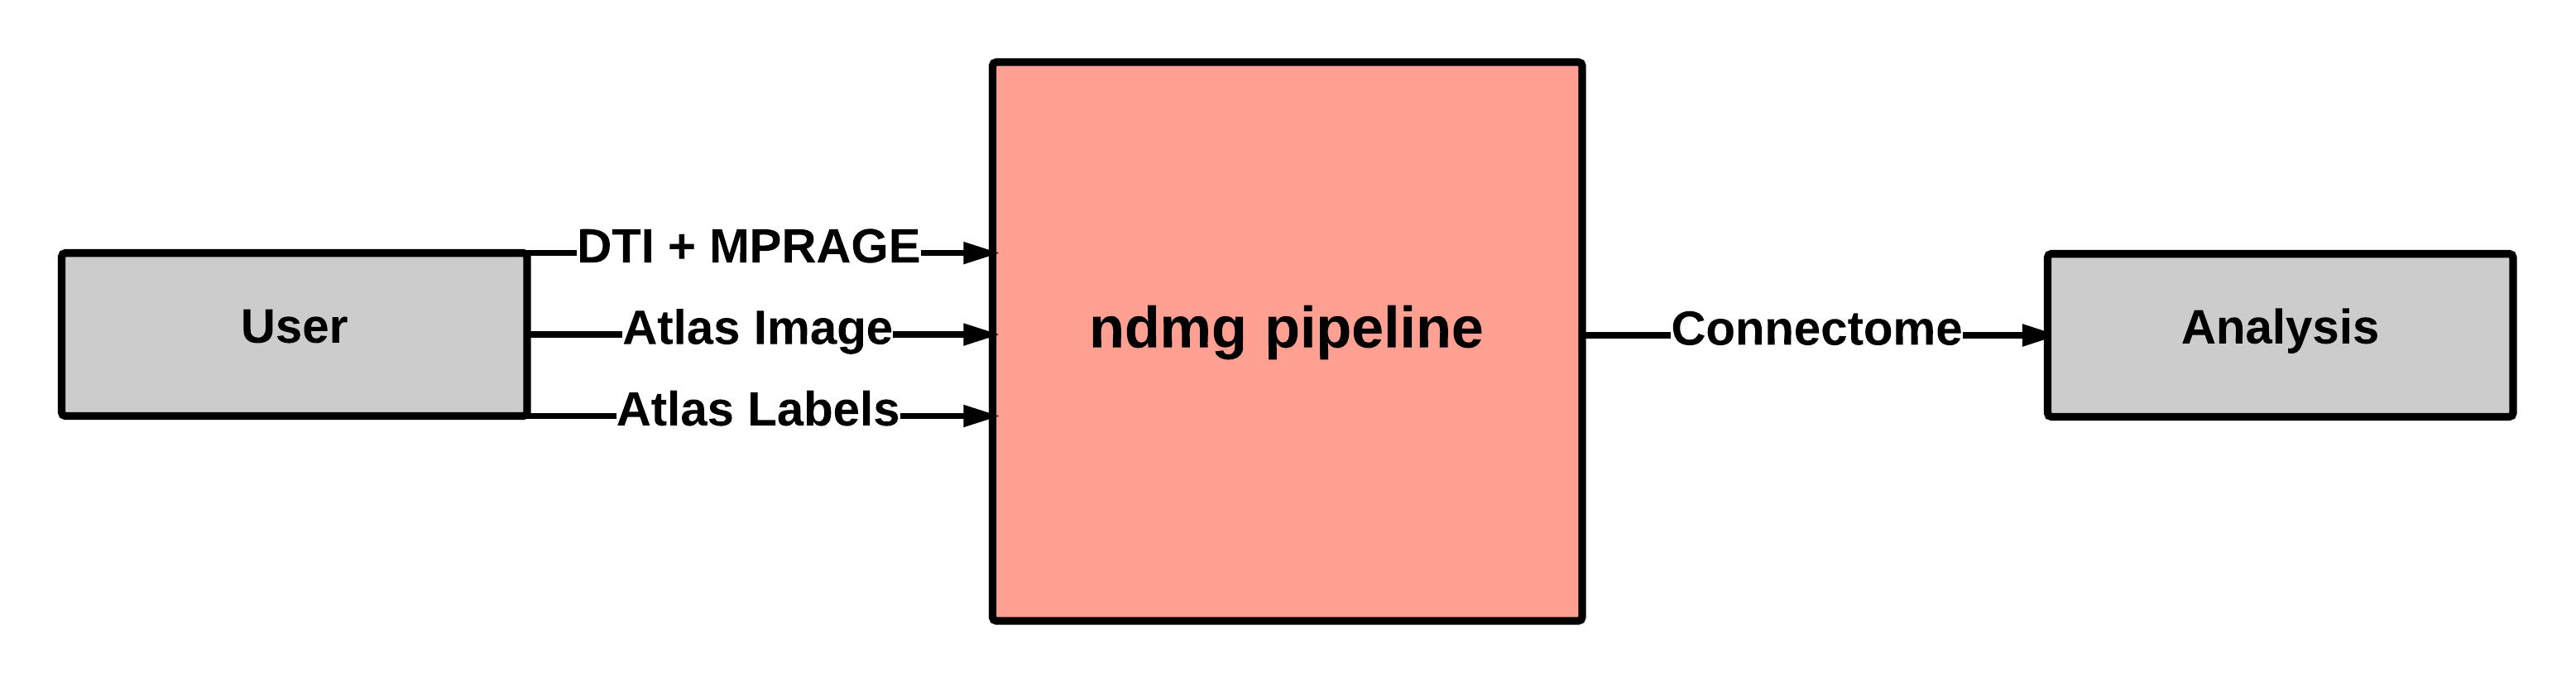
\includegraphics[width=1\textwidth]{./figs/ndmg_simple_pastel.png}
\makeatletter
\let\@currsize\normalsize
\caption{The ndmg pipeline at a high level.}
\label{fig:ndmg-simple}
\end{subfigure}
\begin{subfigure}[h!]{\textwidth}
\centering
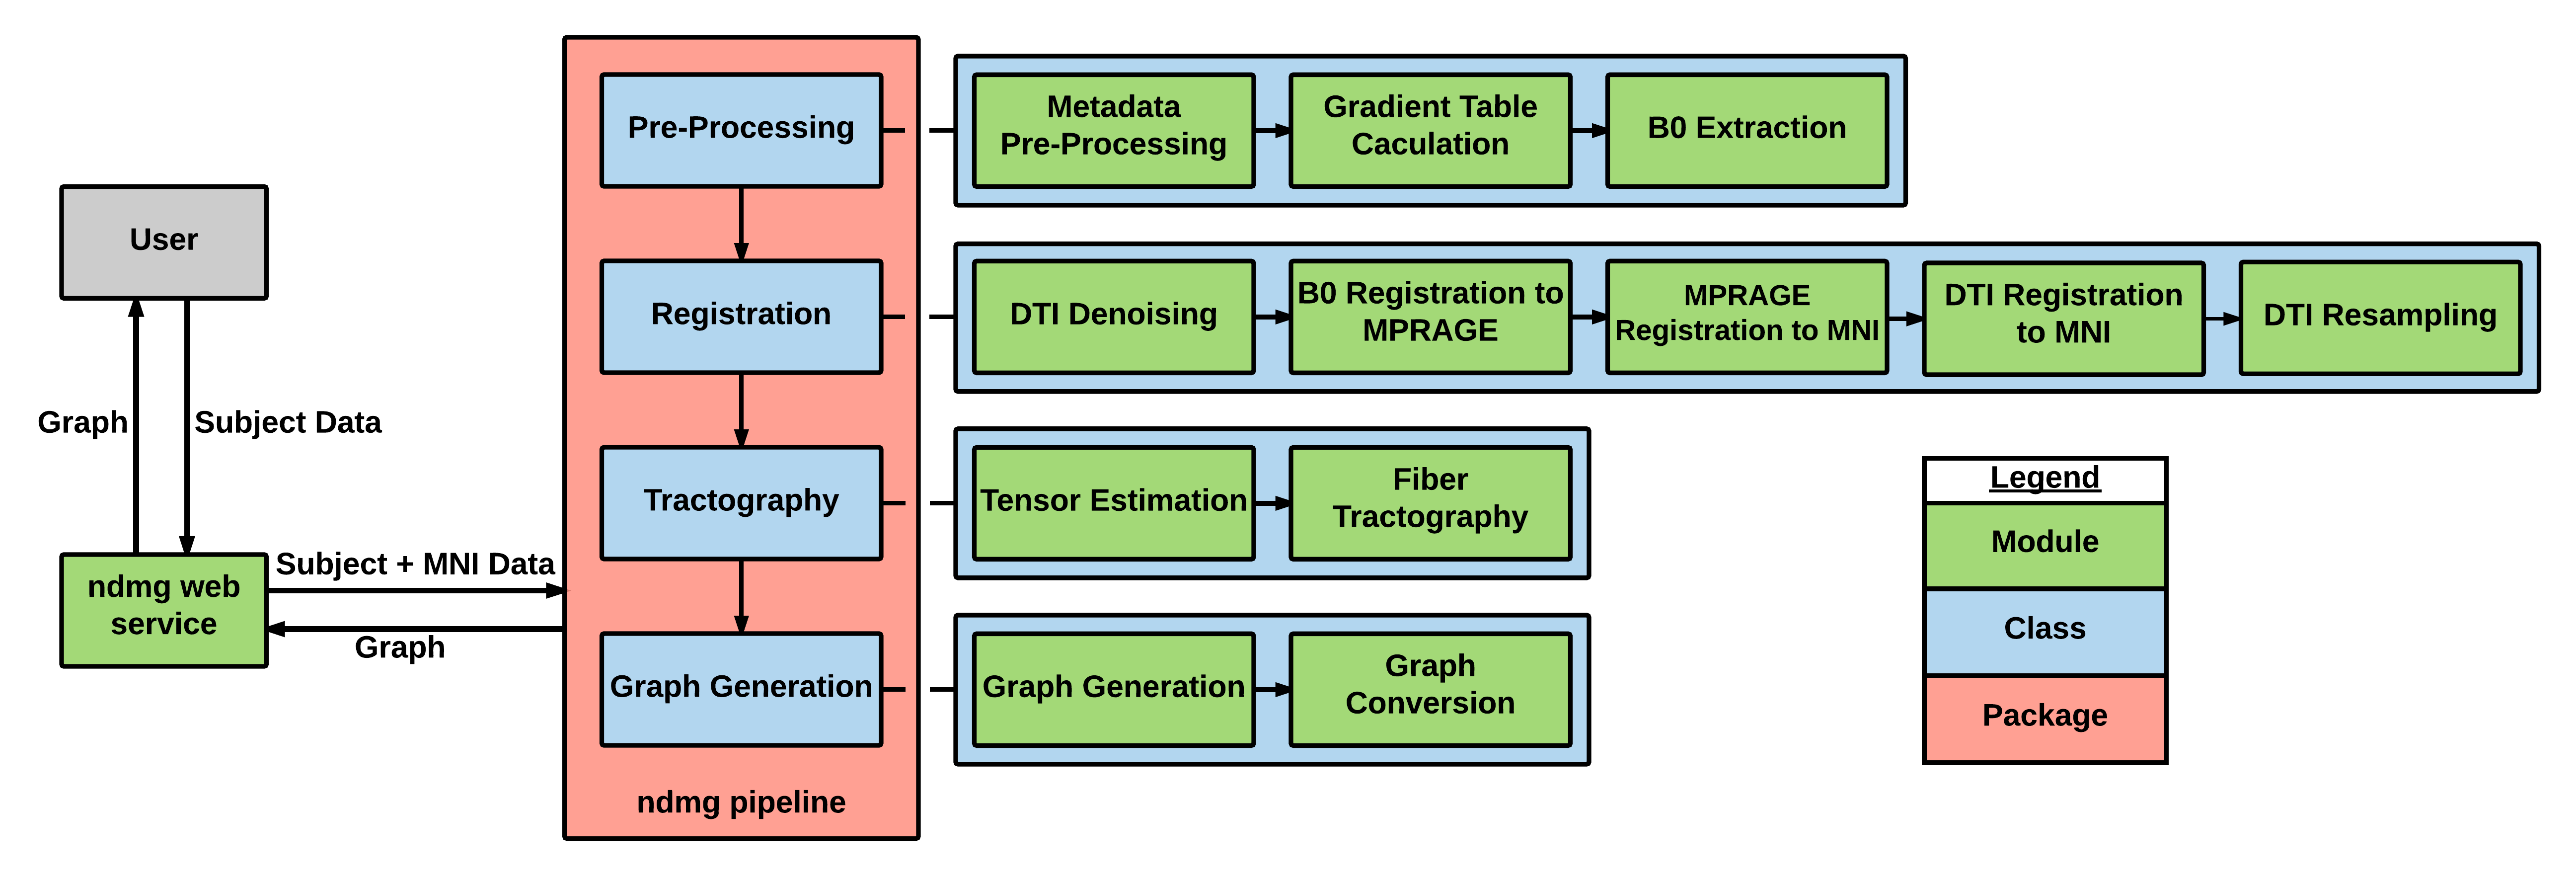
\includegraphics[width=1\textwidth]{./figs/ndmg_pipeline_pastel.png}
\makeatletter
\let\@currsize\normalsize
\caption{The ndmg pipeline as a part of the C4 web service.}
\label{fig:ndmg-pipeline}
\end{subfigure}
\makeatletter
\let\@currsize\normalsize
\caption{High level views of the ndmg MR images to graph pipeline.}
\end{figure}

\section{The ndmg Pipeline}
\label{sec:pipeline}
The ndmg pipeline is an end-to-end tool which reliably estimates connectomes. A user can specify a set of MRI scans and pass them into the pipeline in order to obtain a connectome in return. Further lowering the barrier to entry and enabling ease of use of this pipeline, I have helped to develop a web service entitled C4 (Community Connectomics via Cloud Computing) which has been developed and deployed publicly. Free of charge, users are able to upload their MR image data, press go, and receive a connectome emailed to them in return. A more detailed workflow of this service can be seen in Figure \ref{fig:ndmg-pipeline}. This schematic also highlights the sequence and key set of functions executed in ndmg.

The ndmg pipeline takes two forms of data: subject specific data, and template (often MNI) specific data. Subject specific data consists of images and scan information pertaining to a patient. Template specific data refers to standard reference images and atlases which the subject data can be compared against. The data required can be seen below in Table \ref{tab:datafiles}. Currently, ndmg only supports images in the Nifti1 \cite{nifti} format, and b-value and b-vector files in an ASCII text format. As MR images are produced in other formats such as REC or DICOM, depending on scanner manufacturer, converters exist which will transform these images into the more universal Nifti1 format.
\begin{table}[h!]
\centering
\begin{tabular}{| l | l |}
\hline
\textbf{Type of Data}	& \textbf{Required Inputs} \\ \hline \hline
Subject Specific & MPRAGE, DTI, b-values, b-vectors \\ \hline
Template Specific& template brain, template brain mask, atlas(es)\\ \hline
\end{tabular}
\makeatletter
\let\@currsize\normalsize
\caption{Input data for ndmg.}
\label{tab:datafiles}
\end{table}

Input data undergoes four major transformations from raw image volumes to becoming a connectome: pre-processing, registration, tractography, and graph generation. We will discuss the steps undergone in each in of these transformations, and explain any choices as they come up.

\subsection{Pre-Processing}
\label{sec:preproc}
Prior to complex analysis and transformations of our image data, it is necessary to do some data munging on our images to ensure that more complex operations downstream succeed. We have designed ndmg such that the user does not need to specify any parameters, but of course this requires inferring details from the data itself. The first step of the pre-processing sub-pipeline is metadata pre-processing. In order to acquire DTI images, many gradient fields are applied in varying directions prior to image acquisition. The orientations of the planes defined by these gradients are given in a so-called gradient/b-vectors file, and the intensities of the gradients is given in a b-values file. If the image was acquired with $D$ diffusion directions, the gradient file will contain a $D \times 3$ dimensional matrix, and the b-values file a $D$ dimensional vector. Here we ensure that these files are in the proper orientation and intensities are normalized such that DiPy's gradient table tool (used next) properly interprets the data. The gradient table calculation then simply combines the gradient and b-values files into a data structure that is convenient for querying and analyzing.

The final pre-processing step is extracting the so-called B0 volume from out DTI image stack. When acquired, at least a single 3-dimensional volume of the DTI image has been collected with \textit{no} additional gradient (though technically there exists some small additional field, it is negligible in intensity as compared to the other volumes so considered to be of 0 intensity). The image collected at the location which corresponds to B0 is the DTI volume which most closely resembles the MPRAGE scan, and thus is extracted from the stack and saved for later use.

\subsection{Registration}
\label{sec:reg}
In order to compare analyses across subjects, we must process data in a consistent coordinate system. The space we will refer to here is defined by the MNI152 atlas \cite{mni152}. As we do not know what space our images were originally acquired in, we must transform them such that they overlap our template in both image and voxel spaces - the difference between these two is defined by an affine transform associated with the image as provided by the scanner. As registration of two distinct objects is an inherently imperfect procedure, it is necessary to perform these operations in such a way that there is minimal noise/error introduced. The general principle we will follow involves a series of alignments of \textit{like} images. The process described below is summarized in Figure \ref{fig:ndmg-registration}, and may be useful for following along.
\begin{figure}[h!]
\centering
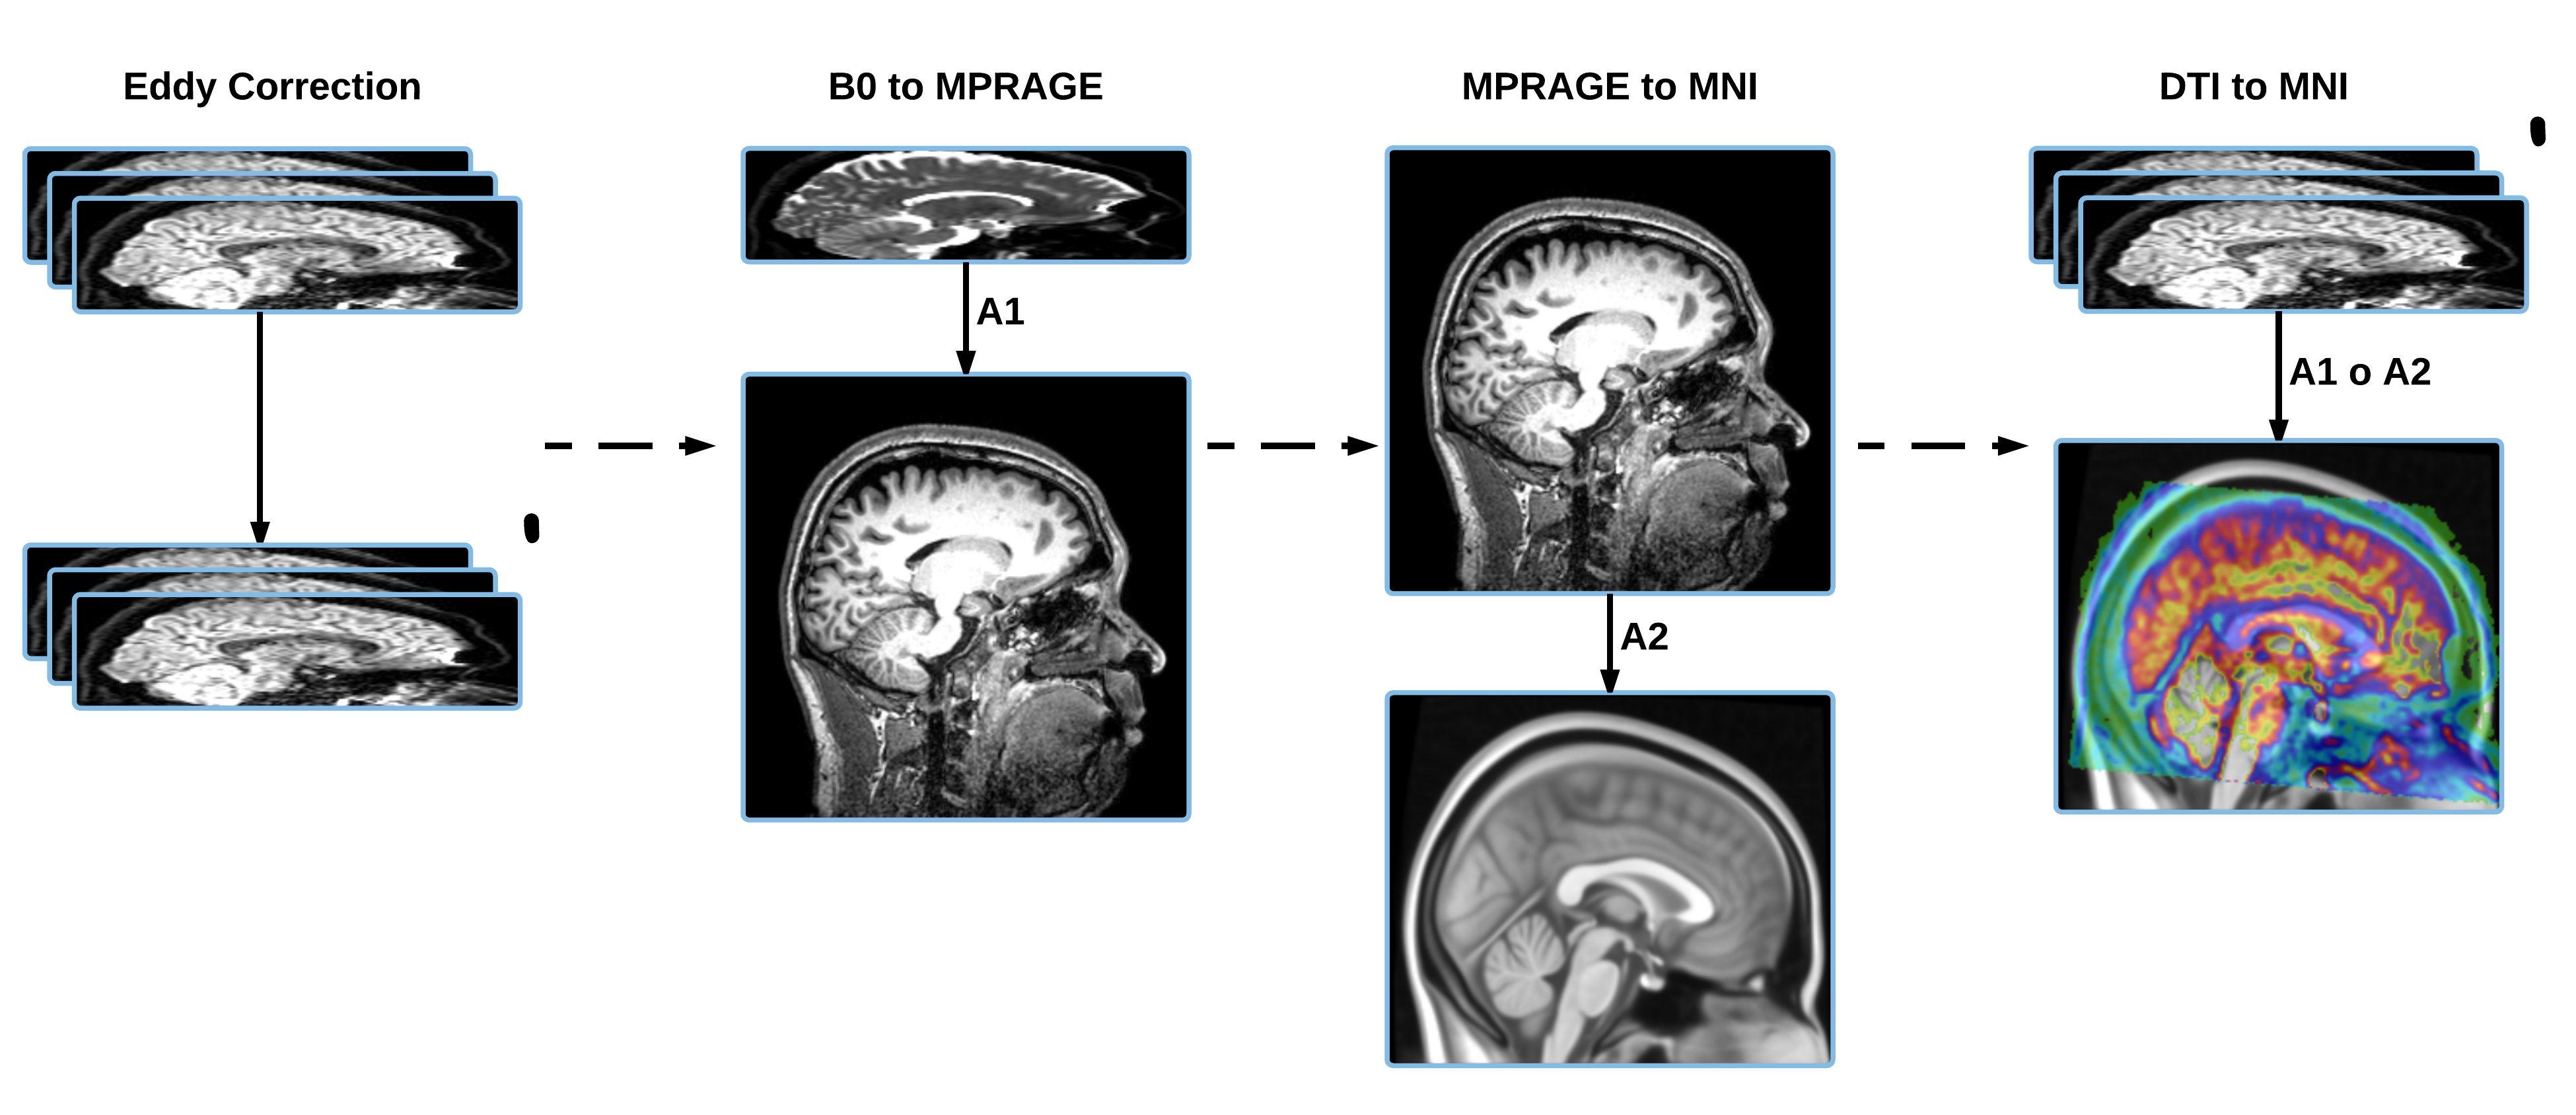
\includegraphics[width=1\textwidth]{./figs/ndmg_registration.png}
\makeatletter
\let\@currsize\normalsize
\caption{Registration sequence used in ndmg.}
\label{fig:ndmg-registration}
\end{figure}

The first alignment we consider is that of individual DTI volumes. As discussed, DTI images are a D-length sequence of 3-dimensional images. As these images were acquired sequentially, there is a high probability that the subject may have shifted slightly between scans, resulting in non-perfectly-overlapping volumes. Also, unrelated to alignment but inherent to MRI, different noise appears in each of these volumes in the form of eddy currents. Eddy currents are circular loops of current which are induced on the surface of tissue within a subject when experiencing a magnetic field. As the gradient applied for each image differs, the eddy currents experienced will also differ. FSL's eddy current correction module handles both the self-alignment and eddy current removal, and thus is applied to obtain a denoised and self-aligned DTI stack. Here we have transformed \textit{like} scans within a modality to one another.

In order to transform our data further, and ultimately into the template space, we must again align \textit{like} images. Using FSL's FLIRT linear registration, we align the previously extracted B0 volume to our subject's MPRAGE scan, as well as the MPRAGE scan to our template volume. This sequence is important, as we are never aligning images which are different in more than 1 way. In the first case, we align images across modalities within our subject, and in the second we align images across subjects but within modalities. At the end of these registrations we store the transform computed, and ultimately combine them.

We are then able to apply this combined transform to our denoised and self-aligned DTI image stack, resulting in an aligned DTI volume that exists in our template space. The final step of our alignment ensures that the registration exists in both our image and voxel space. FSL processes these images in their image space (with consideration of the affine transform in their header), but some other tools do not consider this and treat data as purely data matrices. Resampling our image performs this final alignment in voxel space so that now, regardless of domain, our data is unambiguously aligned to the template.

\subsection{Tractography}
\label{sec:track}
The tractography step is where the DTI-specific techniques come into play, as opposed to more standard image registration or graph construction. The first step in the tractography sub-pipeline is tensor estimation.  Here, we turn the 4-dimensional DTI volume into a 3-dimensional tensor image (i.e each voxel is defined by a tensor rather than an intensity). A tensor is represented by three eigen vectors, one in each of the principal coordinate frame axes.

\begin{figure}[h!]
\centering
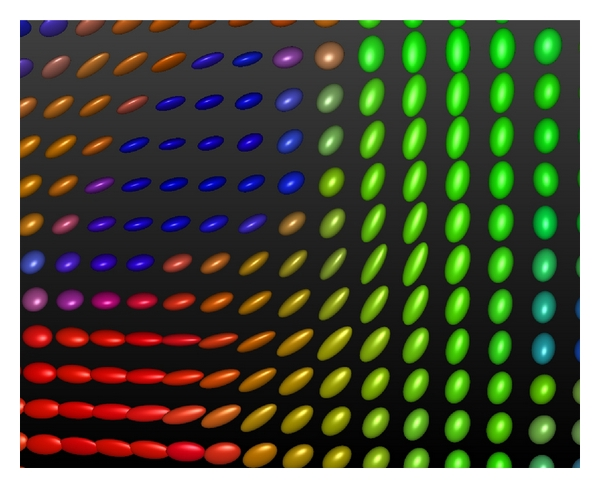
\includegraphics[height=60mm]{./figs/tensors.jpg}
\makeatletter
\let\@currsize\normalsize
\caption{Graphical representation of tensors derived from a diffusion image \cite{van2011cuda}.}
\label{fig:tensors}
\end{figure}

If the intensity along each axis is equal, the tensor would appear as a sphere, whereas if one direction dominates the others it would look sharp like a line along the dominating direction. Shown in Figure \ref{fig:tensors} is a representation of what a slice of a tensor image may look like for a DTI volume. The tensors were calculated using DiPy's diffusion processing package for Python. The degree to which directed flow is believed to exist within a voxel is through a measure called fractional anisotropy. Fractional anisotropy is the ratio of the largest eigen value to the sum of all eigen values. If the anisotropy is close to 1, then flow is heavily favoured in the direction of the eigen vector corresponding to the largest eigen value. As this value decreases, the strength of directed flow also decreases.

Once a tensor image was obtained, the next step was to perform tractography. Going back to the analogy provided above in which we described connectomics as dropping pins and placing threads, the tractography step assumes every voxel in your image is a pin, and spreads threads outwards from each of them. Then, during graph generation stage, we decide which pins we truly care about and downsample or group our fibers accordingly. A set of fiber streamlines can be seen in Figure \ref{fig:fibers}. The tractography method used here is DiPy's EuDX \cite{eudx}. EuDX, much like the Susumu Mori's renowned FACT algorithm \cite{fact}, is a deterministic method for tractography which follows highly asymmetric tensors (i.e. those with strongly directed flow) until some stopping criterion is met. In this case, that stopping criterion is either the strength of the tensor is too low, or the branching angle between adjacent tensors along the fiber being traced is too large. We set each voxel within the brain to be a seed point (i.e. starting point for a fiber), and trace until we are required to stop. Once tractography is complete, we have a dictionary of streamlines which can be traversed and converted into a graph representation of a connectome.
\begin{figure}[h!]
\centering
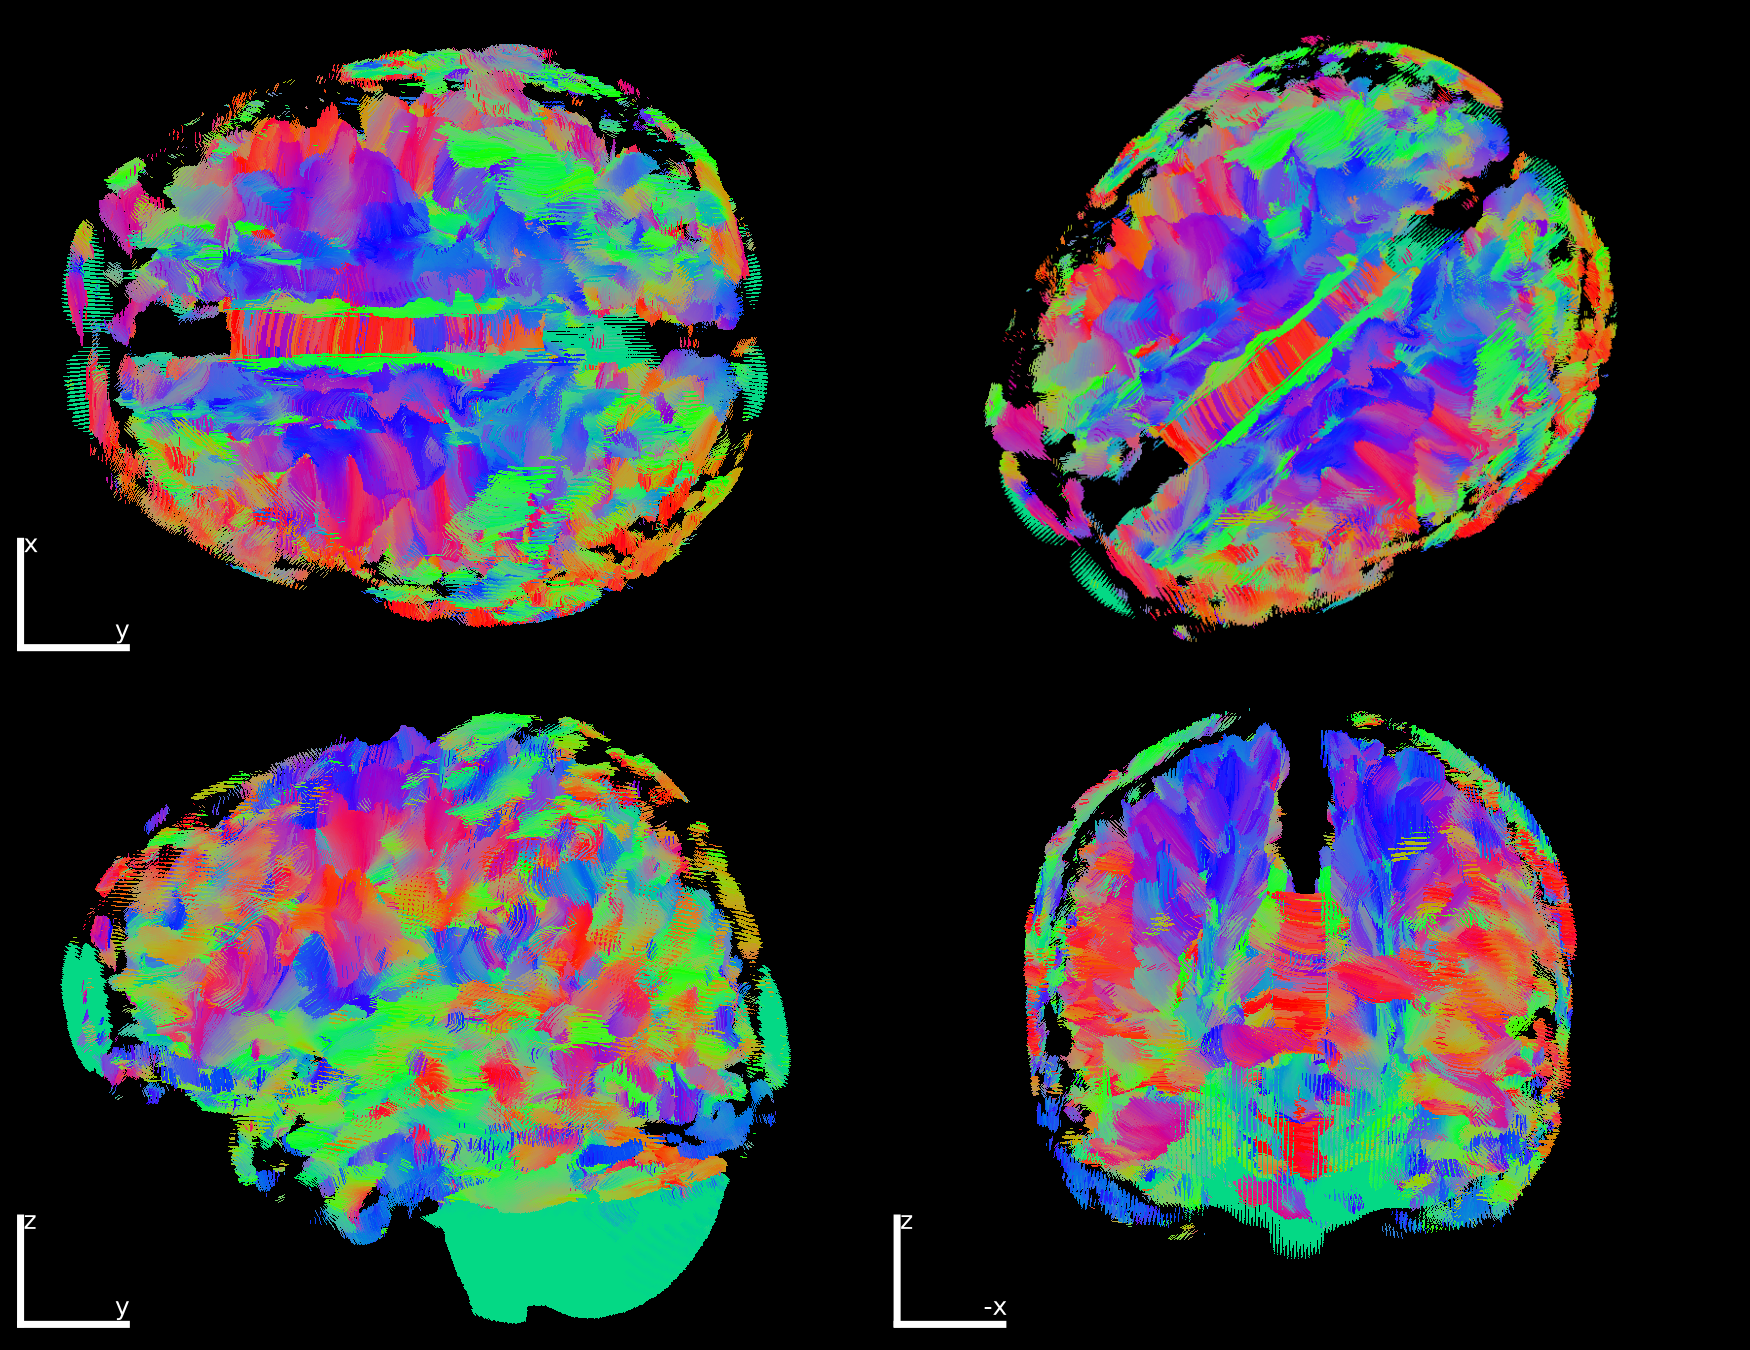
\includegraphics[width=0.9\textwidth]{./figs/3dfibers.png}
\makeatletter
\let\@currsize\normalsize
\caption{Fiber streamlines derived from diffusion tensors, visualized with DiPy.}
\label{fig:fibers}
\end{figure}

\subsection{Graph Generation}
\label{sec:graph}
The final step in our pipeline is the creation of a graph from fibers/streamlines. Utilizing the all-Python library Networkx \cite{networkx} to construct our graphs, we iterate through this procedure for all sets of labels/atlases given.
\begin{figure}[h!]
\centering
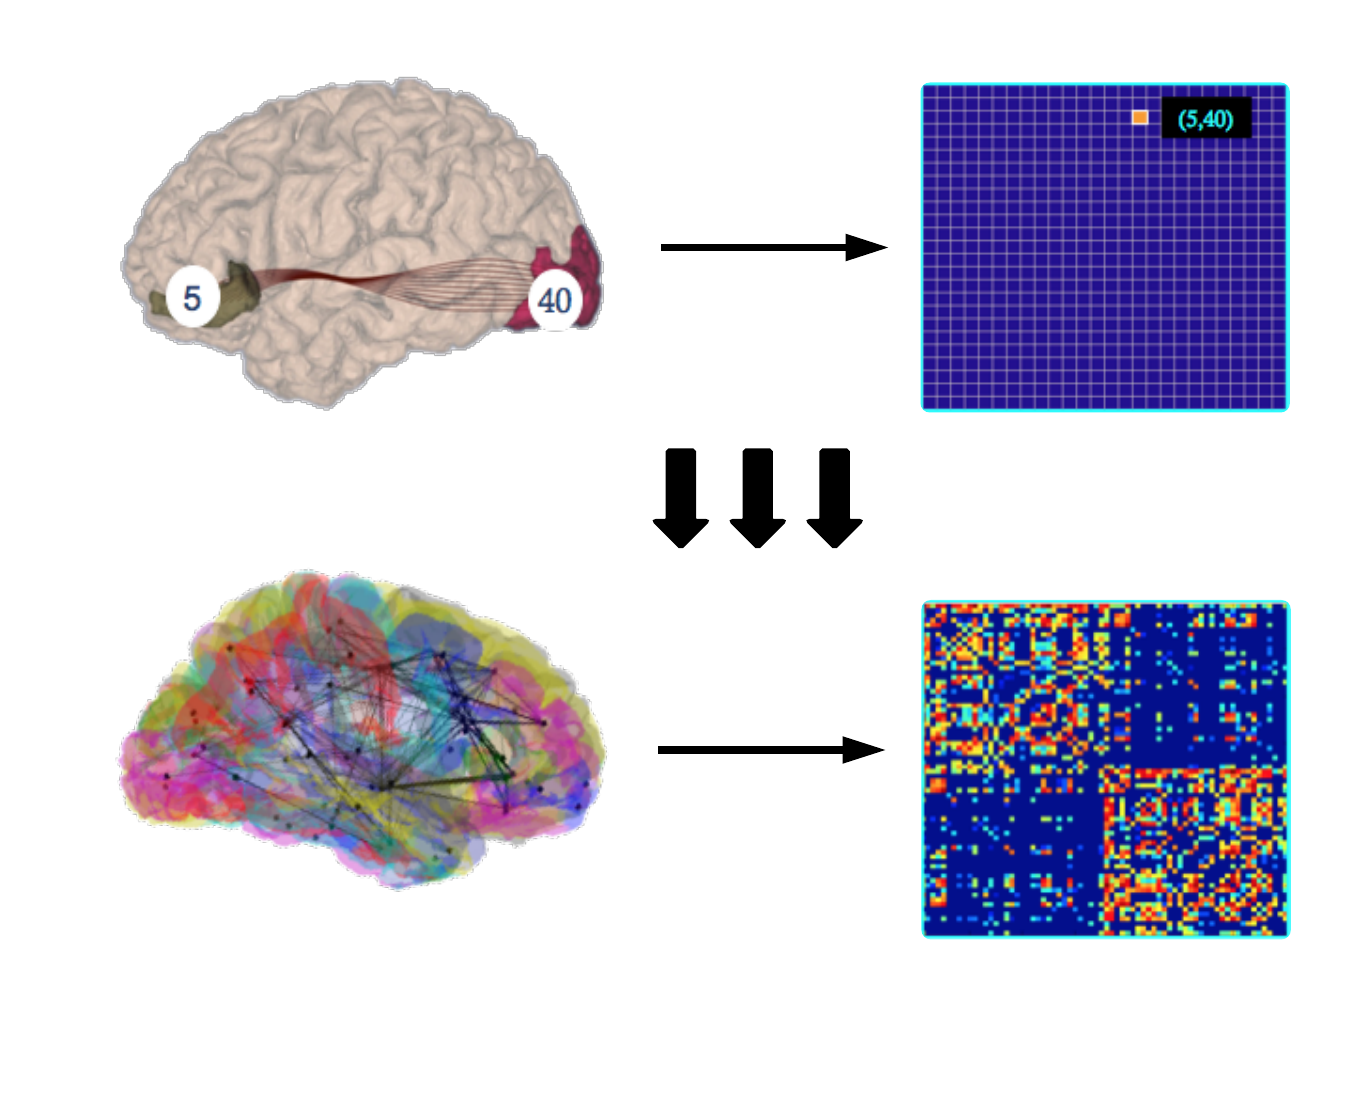
\includegraphics[width=0.8\textwidth]{./figs/graphgen.png}
\makeatletter
\let\@currsize\normalsize
\caption{Graph generation process from fibers \cite{lattman2011}.}
\label{fig:graphgen}
\end{figure}

For each atlas, we iterate through all fibers and trace which regions of the brain they pass through. At the end of each fiber, we take the set of unique regions of interest (ROIs), and add an edge in the graph for all combinations of ROIs. This process can be seen illustrated in Figure \ref{fig:graphgen}.The algorithm takes all fibers that leave the brain and excludes them entirely from the graph, as we know that we should not expect fibers outside of the region defined by a mask of the brain. Once all streamlines have been processed and added to the graph, we populate the graphs with metadata such as pipeline version, and attributes of the ROIs used (if provided). Finally, we save out the graph to our graph database, or in the case of the user running our software, to disk in a compressed format by default. The graph can be output in the popular graphml or edgelist formats, as well, enabling easy analysis of the graphs produced by almost any graph toolbox or programming language.

\subsection{Alternative Processing Methods}
\label{sec:altproc}
We recognize that there were many options for algorithms or implementations at each of the processing steps above. For instance, an alternative to FSL's linear registration would be their non-linear registration. Many other implementations of various processing steps were tested, including tools such as Camino, ANTs, JIST, and others. The choices made were based on design goals kept in mind when designing this tool: open-source, scale-able, short computation time, reliable, and easy to use (minimal dependencies). All design choices were made with regards to these goals, and thus some preferred alternatives for one category such as reliability were not selected because of their lacking in another, such as computation time or adding complicated dependencies. One such example is FSL's probabilistic tractography, which though a more complex and widely recognized tractography algorithm, takes many hours to complete as compared to DiPy's EuDX tractography which can complete in minutes, and, as seen in Section \ref{sec:validate}, produces derivatives with adequate reliability. This logic was also applied to additional processing steps which you have not seen in this manuscript, such as skull stripping, which was found to add more time and reduce reliability of our derivatives as compared to the non-skull stripping alternative.

\section{Architecture of the ndmg Package}
\label{sec:arch}
The ndmg package is not solely a reliable pipeline, but also consists of several classes which group functions and tools based on common purpose. Figure \ref{fig:ndmg-architecture} illustrates this structure and nesting of functions.
\begin{figure}[h!]
\centering
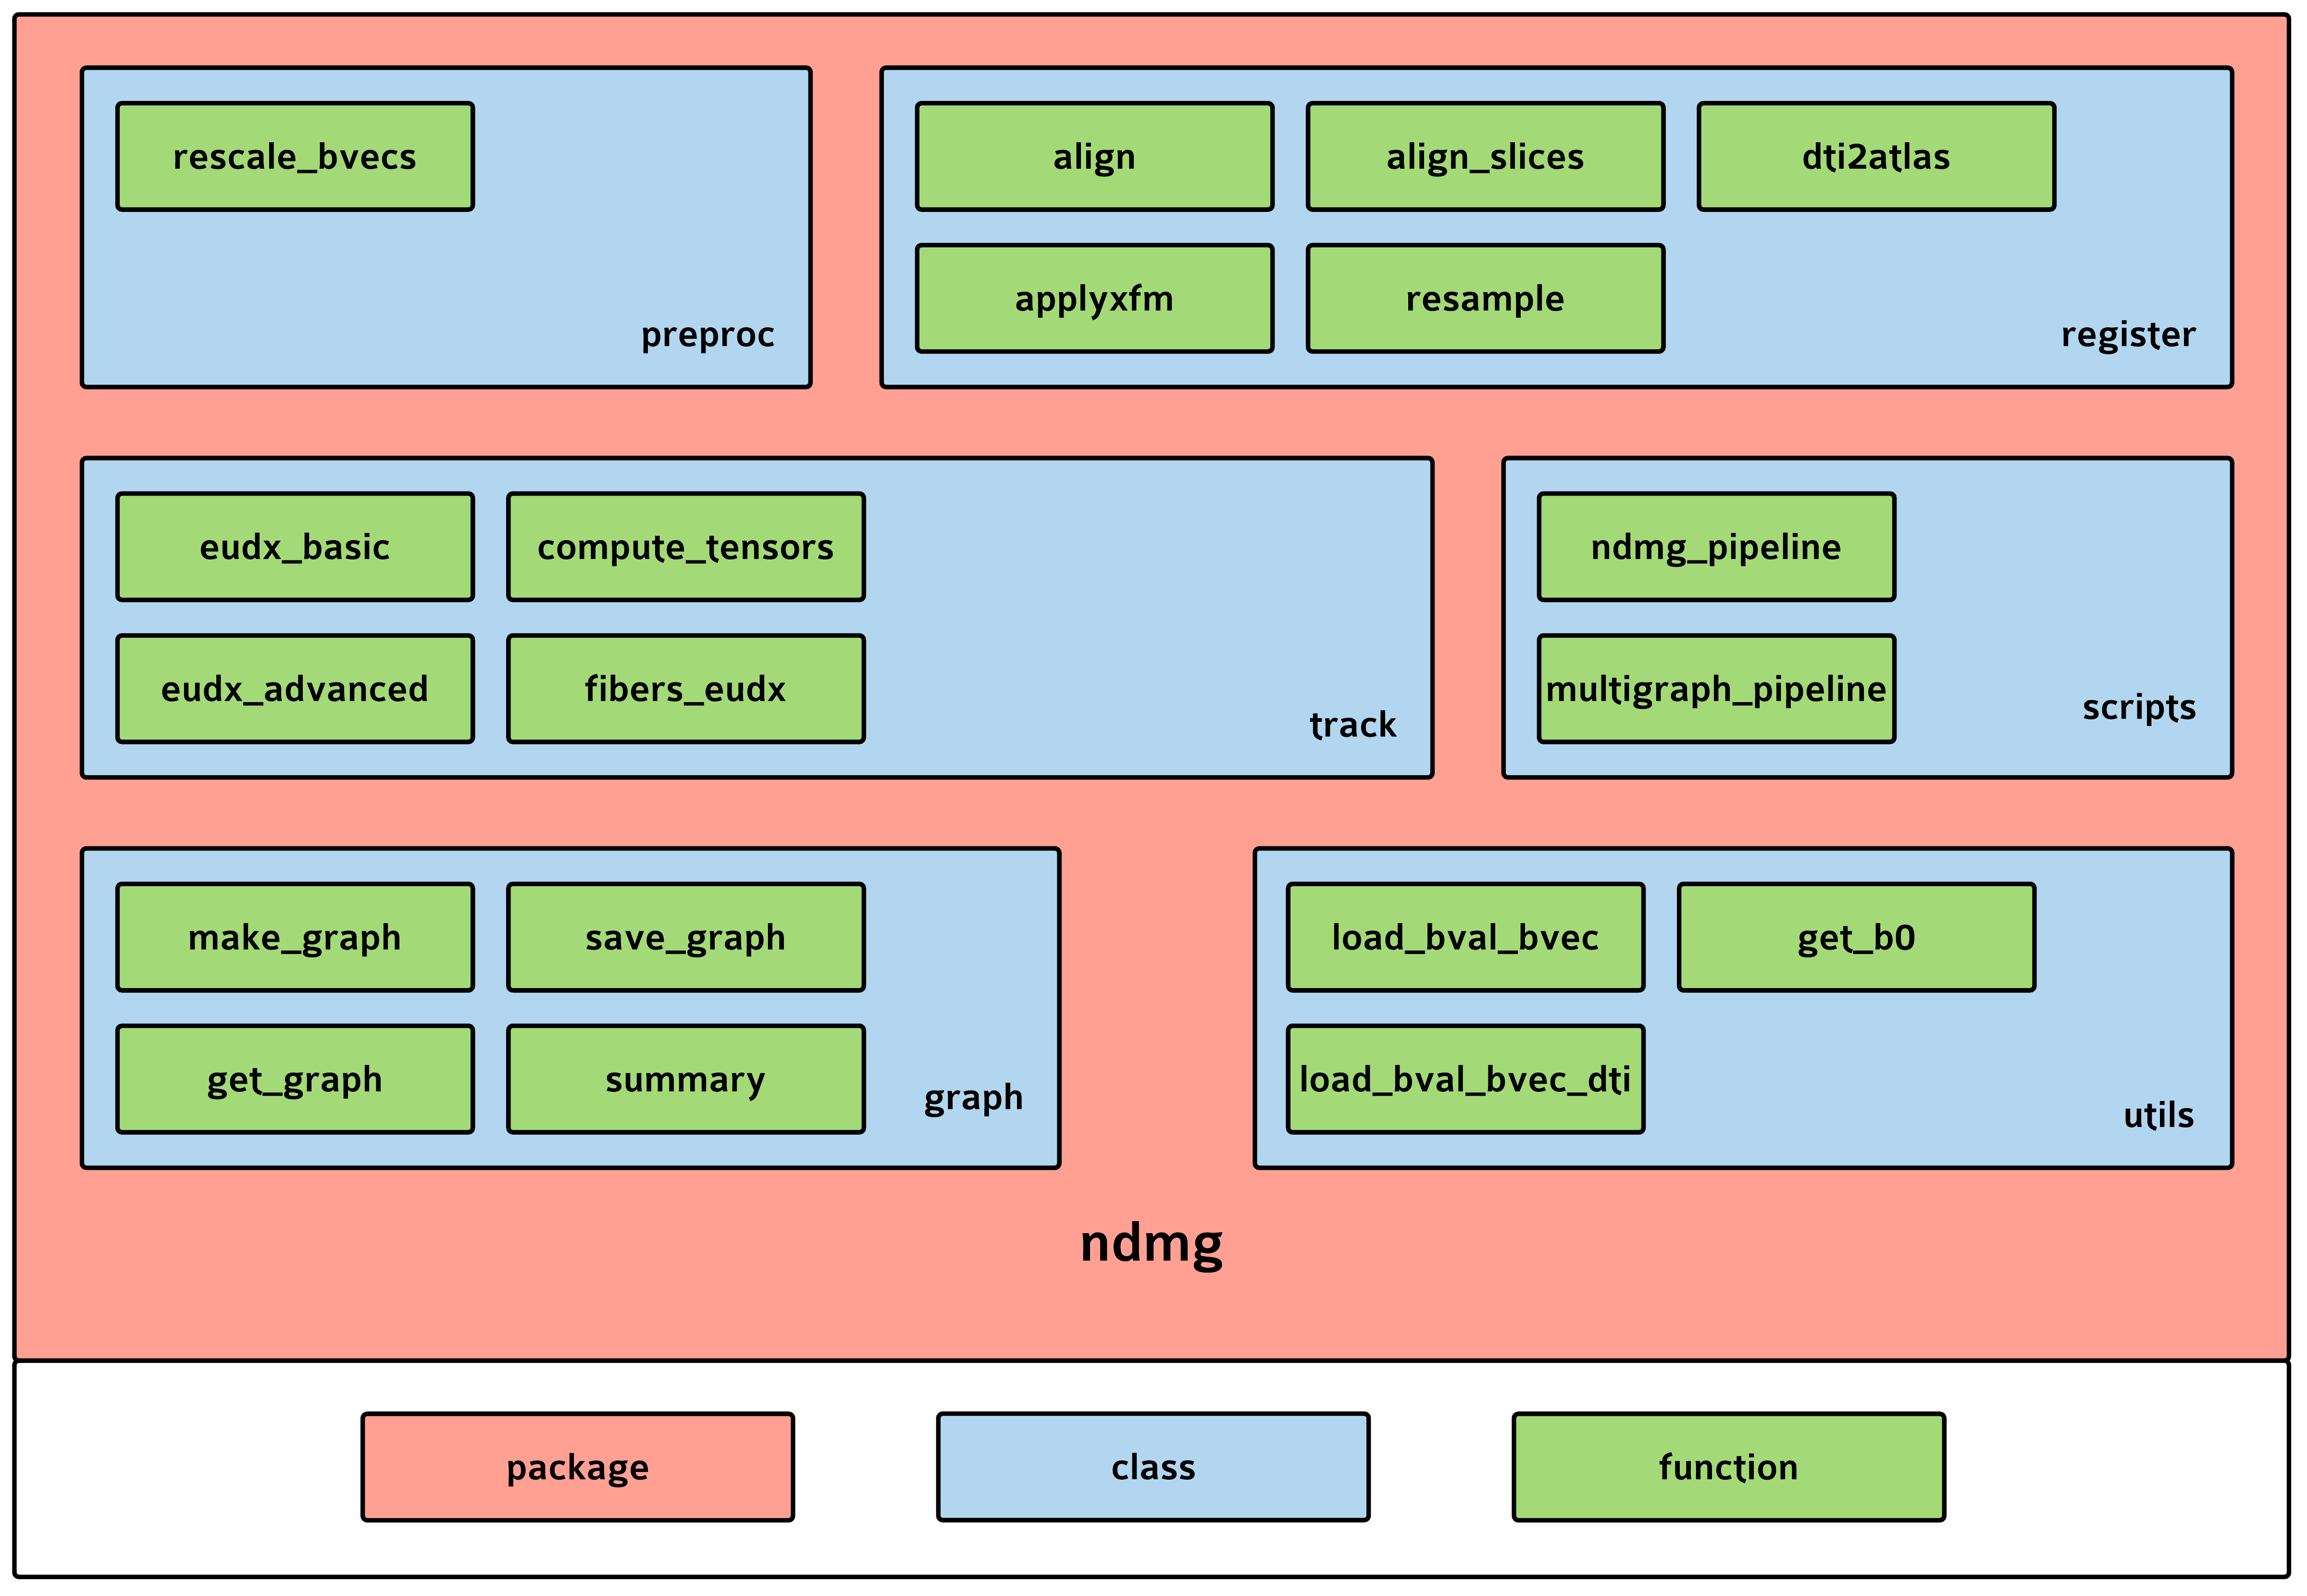
\includegraphics[width=0.97\textwidth]{./figs/ndmg_architecture_pastel.png}
\makeatletter
\let\@currsize\normalsize
\caption{Package architecture of ndmg.}
\label{fig:ndmg-architecture}
\end{figure}
The ndmg package consists of 8 main classes: preproc, register, track, graph, scripts, stats, navigate, and utils, many of which contain functions which were discussed in Section \ref{sec:pipeline}. Functions coloured in green exist, and those in yellow are planned but not yet implemented. Each class and method is described and defined at \url{http://docs.neurodata.io/ndmg/py-modindex.html}.

\section{Validation}
\label{sec:validate}
In order to ensure the derivatives produced by ndmg were meaningful, we validated our pipeline through repeated trial analysis and a metric entitled discriminability. Many datasets available contain multiple scans from the same subjects - these are called test-retest datasets, and enable our repeated trial analysis. We assert that the connectome estimated from one subject on a given day (from a given scan) will be more similar to their own connectome as measured at another time, than it will be to anyone else's connectome. Discriminability, shown in Equation \ref{eq:descr}, is the probability that within a given dataset, a subject's nearest most similar connectome will be their own from a separate scan. Here, $a$ is the adjacency matrix of their connectome, $i$ represents the subject id, and $j$ represents the scan id, and $\Vert  \Vert_F$ represents the Frobenious norm. 
\begin{equation}
P(\Vert a_{ij} - a_{ij'}\Vert_F \leq \Vert a_{ij} - a_{i'j''}\Vert_F)
\label{eq:descr}
\end{equation}
A perfect discriminability score is 1, as that means that every subject was correctly matched to their corresponding scan. It is worth noting that this validation is only possible on test-retest datasets, and thus cannot always be used to assess performance of ndmg. The benefit to using discriminability is that, as shown in an in-development paper being led by Shangsi Wang \cite{swang2015}, optimizing discriminability optimizes the lower bound of predictive accuracy. This is to say that, as you improve the discriminability of a tool, you are effectively improving the expected worst possible outcome of said tool. In the case of ndmg, we have used this metric to assess the quality of our lower bound of predictive accuracy over various processing strategies, algorithms, implementations, and machines. 

The discriminability was computed on graphs with three different types of edge weighting: raw edges, the log of raw edge values, and ranked edges. Passing to ranks takes the edge with the largest magnitude and assigns it the highest possible rank for that atlas, given by $\binom{N}{2}$. This operation is performed for all edges in sequence, where ties are settled by averaging all ranks in the tie. For the log edge weights, the natural logarithm is used.

\section{Quality Control}
We performed quality control on our data at two stages: raw images, and graphs. The purpose of this control was to observe the potency of batch effects in our data, as well as learn features about our data which may help guide future analyses.

\subsection{Raw Data}
In order to anticipate the prevalence of batch effects in our produced graphs, we visualized the distribution of voxel intensities in our image data. When comparing our raw image data, it was important to compare elements which would be maximally similar, and relevant in the operation of the pipeline. The MPRAGE scans, though the highest quality, were not necessarily acquired during the same session as the DTI scans, and are too far removed from the actual DTI data upon which processing takes place. The DTI volumes undergo gradient fields which are not necessarily of constant magnitude or direction across subjects or datasets, and thus difficult to compare. This leaves the B0 volume of the DTI stack, as it experiences no additional gradient field from the bulk magnetization, and thus looks the most like a structural scan but is invariant to many of the DTI acquisition parameters such as gradient intensity or direction.

For each dataset we computed histograms and then kernel density estimates of the B0 volume corresponding to each DTI session. These probability distribution functions (PDFs) were then plotted side-by-side so that differences may be easily observed.

\subsection{Graphs}
As discriminability validation is limited to test-retest datasets, we have chosen several other statistics to compute upon the graphs which will give insight into their structure and consistency. The metrics we evaluated were: clustering coefficient; number of non-zero edges; betweenness centrality; degree sequence; and, edge weight distribution. Important in developing a scalable tool which can be processed across many different datasets, is robustness in the graphs produced. These metrics were selected in order to obtain a general summary of the graphs, and enable us to evaluate non-test-retest datasets by comparing them to datasets upon which we could compute discriminability.

If our graphs can be represented as $G = (V,E,W)$, where $V$ is the set of vertices and $E$ is the set of edges, with $W$ being the weights associated with each edge. Then, $e_{ij}$ denotes an edge that connects nodes $v_i$ and $v_j$. As our graphs are undirected, edges are symmetric (i.e. $e_{ij} = e_{ji}$). The neighbourhood of a vertex $v_i$ can be denoted as $N_i$. We will explore each of the analyses listed above.

The clustering coefficient (Equation \ref{eq:cc}), provides the fraction of total edges among neighbours of a vertex of interest, $v_i$.

\begin{equation}
C_i = \frac{|\{  e_{jk} : v_j, v_k \in N_i, e_{jk} \in E \}|}{|N_i|(|N_i|-1)}
\label{eq:cc}
\end{equation}

The number of non-zeros counts the number of edges in the graph (Equation \ref{eq:nnz}).

\begin{equation}
NNZ = |E|
\label{eq:nnz}
\end{equation}

The betweenness centrality of a node counts the total number of shortest paths between two other nodes in the graph (Equation \ref{eq:bc}). Here, $\sigma_{jk}$ denotes the number of shortest path between nodes $j$ and $k$, and $\sigma_{jk}(v_i)$ is the number of those which pass through node $v_i$.

\begin{equation}
BC(v_i) = \sum_{i \neq j \neq k}^{|V - v_i|} \frac{\sigma_{jk}(V_i)}{\sigma_{jk}}
\label{eq:bc}
\end{equation}

The degree sequence of the graph is the distribution of node degrees. The degree of a node is given by the total number of edges incident to a node, here equivalent to the neighbourhood of that node (Equation \ref{eq:deg}).

\begin{equation}
deg(v_i) = N_i
\label{eq:deg}
\end{equation}

The edge weight distribution is simply the distribution of $W$ for the graph.

%=========================
%%% End Methods

%%% Begin Results
%=========================
\chapter{Results}
\label{sec:results}
We have created an open-source reliable pipeline and software package for connectome estimation from multi-modal MR images, as well as multiple publicly available services and over $100,000$ connectomes, significantly lowering the barrier to entry for connectomics estimation and analysis.

\section{The ndmg Pipeline \& Package}
\label{sec:resultndmg}
Through ndmg, there now exists an
\begin{figure}[h!]
\centering
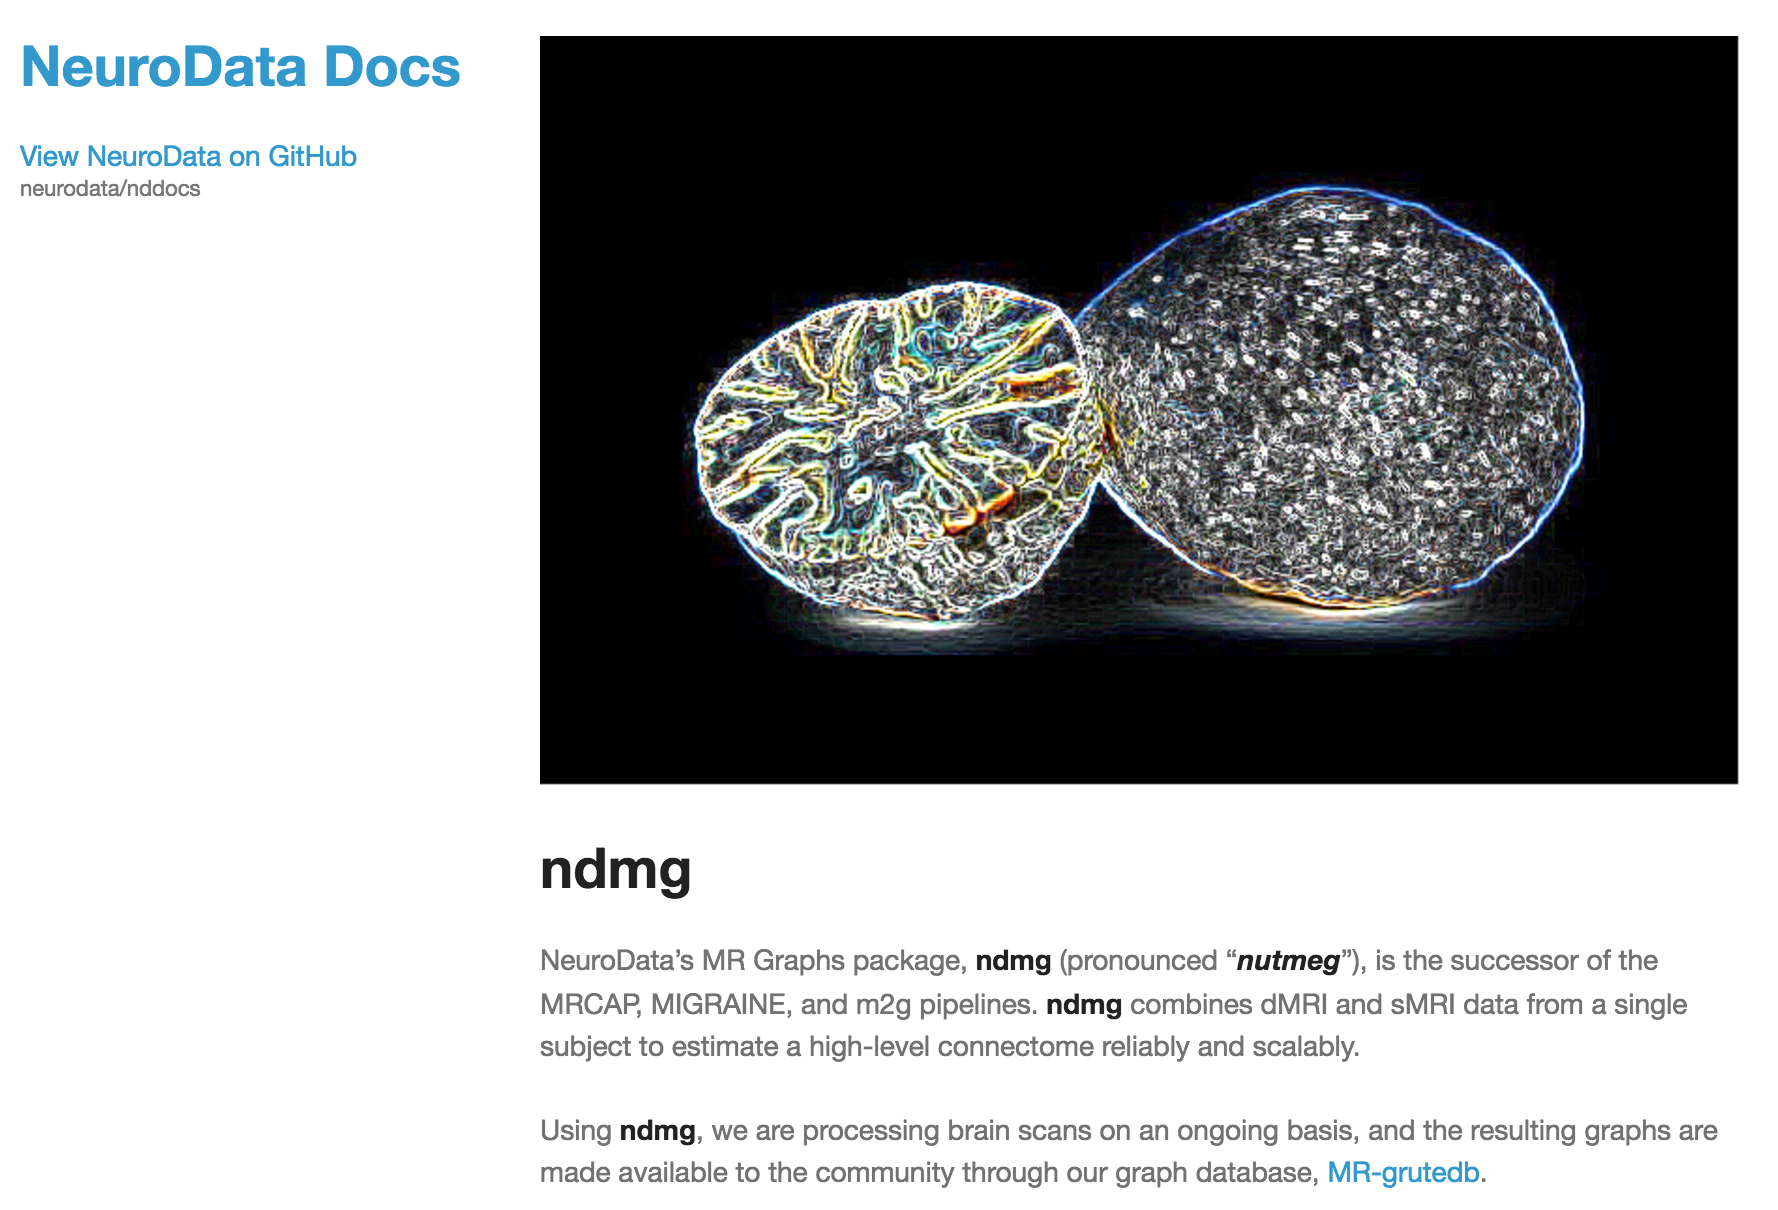
\includegraphics[width=0.76\textwidth]{./figs/website.png}
\makeatletter
\let\@currsize\normalsize
\caption{Screenshot of ndmg documentation and code webpage.}
\label{fig:website}
\end{figure}
extensively documented, publicly available and open source Python package for connectome estimation from MR images. Seen in Figure \ref{fig:website} is the landing page of the package's website, \url{http://m2g.io}. From here, a user may easily download and install the package and pipeline, example data, and estimate connectomes on their personal computer in a matter of minutes.

\section{Open Access Data}
\label{sec:opendata}
Many data collection initiatives exist which have gathered an abundance of MR data. Furthermore, many of these initiatives have also focused on producing publicly available data for the scientific community.
\begin{table}[h!]
\centering
\begin{tabular}{| l | c | c | c |}
\hline
\textbf{Dataset}	& \textbf{Subjects} & \textbf{Scans Per Subject} & \textbf{Total Scans Processed} \\ \hline \hline
KKI2009 & $21$ & $2$ & $42$ \\ \hline
NKI-ENH & $198$ & $1$ & $198$\\ \hline
NKITRT & $24$ & $2$ & $40$\\ \hline
MRN114 & $114$ & $1$ & $114$\\ \hline
MRN1313 & $1313$ & $1$ & $1307$\\ \hline
JUNG2015 & $255$ & $1$ & $254$\\ \hline
SWU4 & $235$ & $2$ & $454$ \\ \hline
BNU1 & $57$ & $2$ & $114$\\ \hline
BNU3 & $48$ & $1$ & $48$\\ \hline
HNU1 & $30$ & $10$ & $300$\\ \hline
HCP500 & $526$ & $6$ & $2843$\\ \hline
\textbf{Total} & \textbf{2821} &  & \textbf{5714}\\ \hline
\end{tabular}
\makeatletter
\let\@currsize\normalsize
    \caption{Publicly available and redistributable DTI+MPRAGE datasets.}
   	\label{tab:data}
\end{table}
\begin{figure}[h!]
\centering
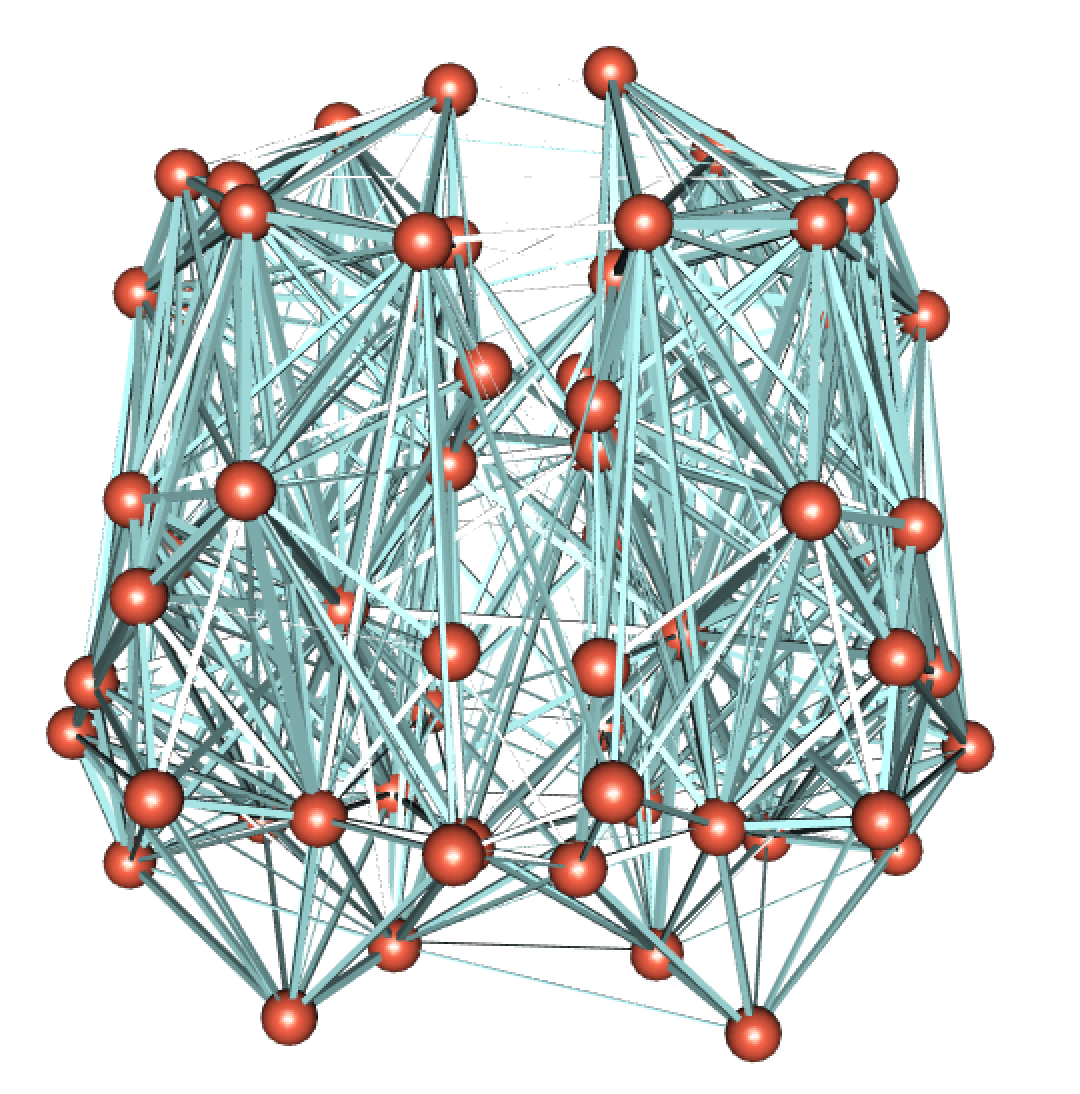
\includegraphics[width=0.45\textwidth]{./figs/graph.png}
\makeatletter
\let\@currsize\normalsize
\caption{Example graph generated by ndmg.}
\label{fig:3dgraph}
\end{figure}

Seen in Table \ref{tab:data} is all known publicly available and redistributable MR data containing both T1 and DTI contrasts. All of this data has been processed using ndmg, and as will be highlighted in Section \ref{sec:mrgrutedb}, the derivatives have been made publicly available for analysis by the community. The Subjects and Scans Per Subject columns indicate the desired number of subjects and scans collected as a part of the study, respectively. The discrepancy in the product of these columns for a given dataset and the Total Scans Processed column is due to incomplete data being distributed or other processing difficulties. Figure \ref{fig:3dgraph} shows an example graph produced by ndmg.


The publicly available connectomes have been generated using a set of 24 atlases of varying scales, and are shown in Table \ref{tab:atlas}. These atlases are defined either physiologically or structurally by neuroanatomists (Desikan \cite{desikan} , Talairach \cite{talairach}, AAL \cite{aal}, JHU\cite{jhu}, HarvardOxford\cite{harvardoxford}), are generated using a segmentation algorithm looking for certain features or groupings (CPAC200 \cite{cpac}, slab1068 \cite{slab1068}, slab907 \cite{slab907}), or are images of the brain which have been cubed-up by our own brain-downsampling code (Voxelwise, ND\#).

\begin{table}[h!]
\centering
\begin{tabular}{| l | c |}
\hline
\textbf{Atlas}	& \textbf{ROIs} \\ \hline \hline
Desikan & 70 \\
Talairach & 1105 \\
HarvardOxford & 111 \\
AAL & 116 \\
JHU & 48 \\
CPAC & 200 \\
Slab907 & 907 \\
Slab1068 & 1068\\ 
Voxelwise & 1827243 \\ \hline
\end{tabular}
\quad 
\begin{tabular}{| l | c |}
\hline
\textbf{Atlas} & \textbf{ROIs} \\ \hline \hline
ND00071 & $70$  \\
ND00096 & $95$ \\
ND00108 & $107$ \\
ND00140 & $139$ \\
ND00195 & $194$ \\
ND00278 & $278$ \\
ND00350 & $349$ \\
ND00446 & $445$ \\
ND00583 & $582$ \\
ND00833 & $832$ \\
ND01216 & $1215$ \\
ND01876 & $1875$ \\
ND03231 & $3230$ \\
ND06481 & $6480$ \\
ND16784 & $16783$ \\
ND72784 & $72783$ \\ \hline
\end{tabular}
\makeatletter
\let\@currsize\normalsize
\caption{Atlases used to estimate connectomes}
   	\label{tab:atlas}
\end{table}

\section{Discriminability of ndmg}
\label{sec:resultdesc}
As described in Section \ref{sec:validate}, the ndmg connectome estimation pipeline was primarily evaluated based on the discriminability of the graphs produced among datasets which enabled repeated trial/test re-test analysis. Shown in Figure \ref{fig:descr} is the performance of ndmg on two of the test-retest datasets shown in Table \ref{tab:data}, KKI2009 and SWU4, over multiple atlases.
\begin{figure}[h!]
\centering
\begin{subfigure}[h!]{0.9\textwidth}
\centering
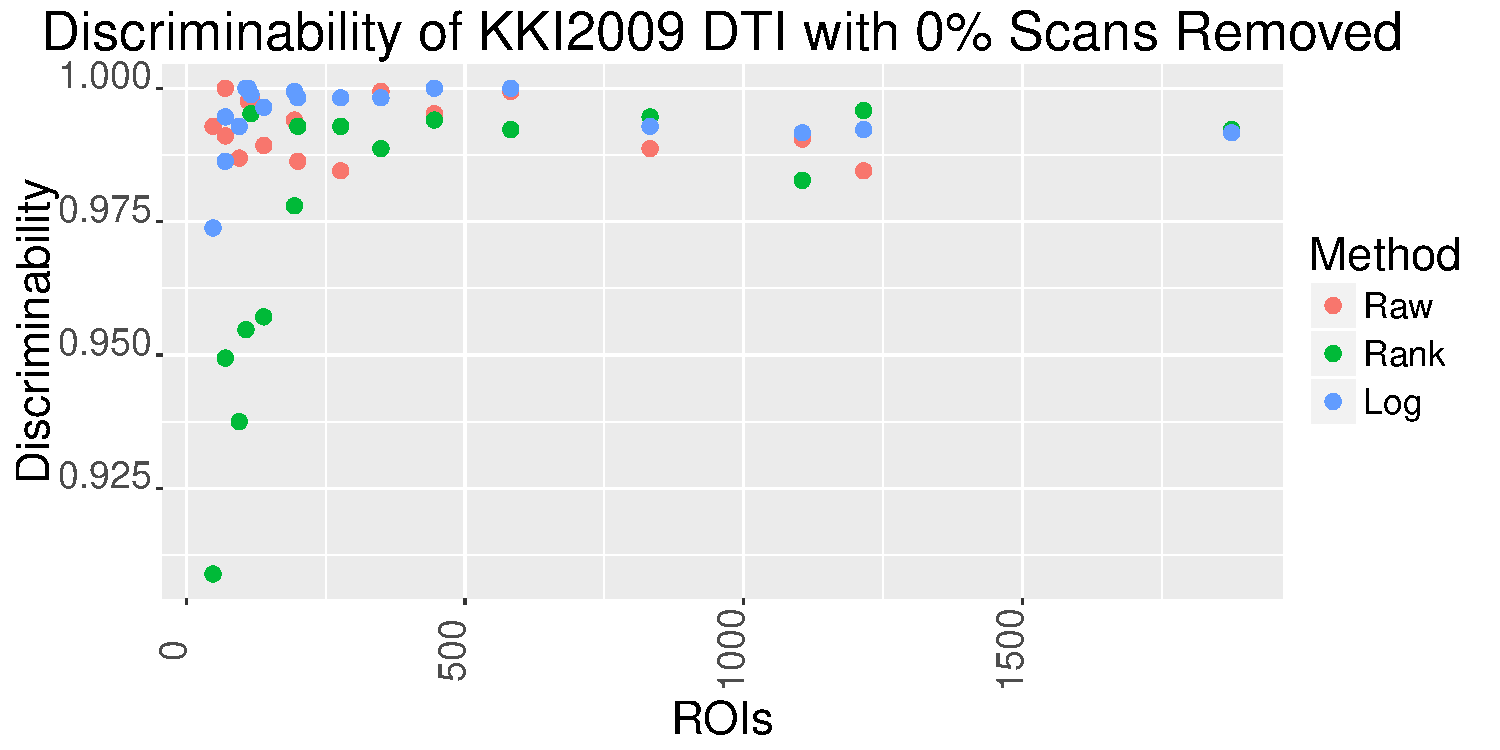
\includegraphics[width=0.9\textwidth]{./stats/kki2009_disc.pdf}
\end{subfigure}
\begin{subfigure}[h!]{0.9\textwidth}
\centering
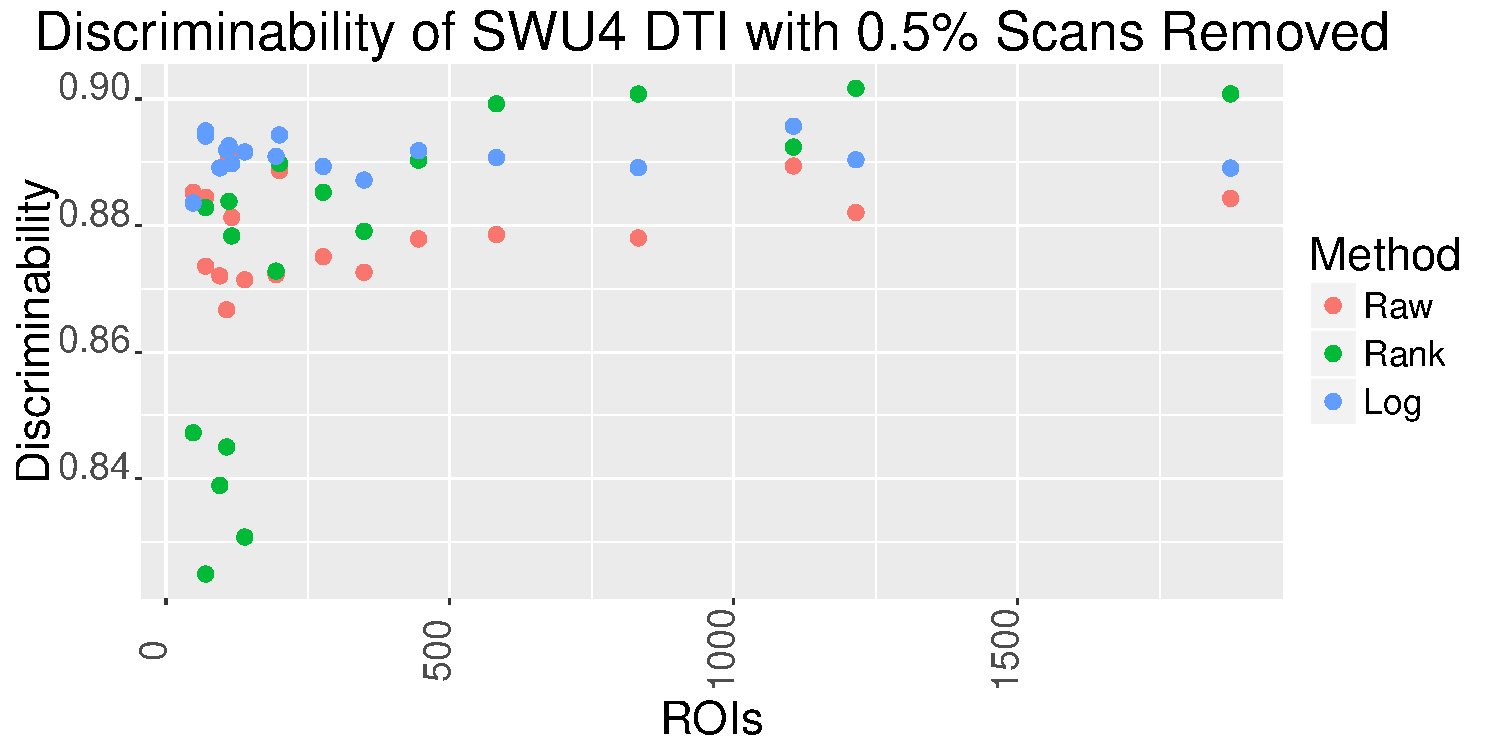
\includegraphics[width=0.9\textwidth]{./stats/swu4_disc.pdf}
\end{subfigure}
\makeatletter
\let\@currsize\normalsize
\caption{Discriminability of populations of connectomes produced by ndmg evaluated for multiple scales.}
\label{fig:descr}
\end{figure}
We can see from this figure that in KKI2009, a dataset with 42 graphs from 21 subjects, for many atlases we obtain a perfect discriminability score, and for all others the discriminability is still above $0.90$. This result is tremendously encouraging, and suggests that as we can pick subjects out of a lineup, downstream tasks such as covariate classification may be possible. We notice that raw and log counts perform consistently across atlases, with log being slightly better, and the rank method performs significantly worse for small atlases and improves as the number of ROIs grow larger. For larger atlases (i.e. a finer resolution parcellation of the brain) we are able to gain resolution in our connectome estimate, but at the cost of an increased impact of voxelwise noise, suggesting why the ranked method performs well at this higher-node operating point. Based on our analysis, we recommend the 1105 node Talairach atlas. This is based on it's strong discriminability performance, relatively large number of nodes, and that the Talairach parcellation is based in neuroanatomy and thus may provide meaningful node information in contrast to those generated by an arbitrary segmentation algorithm.

Similarly, this analysis was performed on the much larger SWU4 dataset, containing 454 graphs from 227 subjects. The discriminability of this dataset is between 0.82 and 0.92 for all atlases. The same patterns observed for the edge weighting method in the KKI2009 dataset hold for SWU4.


\section{Quality Control}
Once we obtained a strong discriminability score and believed our pipeline to be reproducible, we performed further analyses on both the raw images as well as estimated graphs to understand properties of our data.

\subsection{Raw Data}
Data acquired in separate studies have often been collected with widely varying parameters, and there is a real concern for batch effects both in the raw data and the downstream derivatives such as graphs. Figure \ref{fig:b0s} illustrates the histograms of intensity within the B0 volumes of every scan in a dataset, across several datasets. With the exception of the KKI2009 dataset, the intensity range for each dataset is consistent, and even within the KKI2009 dataset the shape of the histograms is consistent though scaled. The NKIENH dataset appears to contain two populations of scans, and this is likely due to a change in the field of view of the scanner when acquiring the images, a process that would be done when imaging the smaller head of a child as compared to an adult. Despite these differences, it appears as though our input data has remarkably small batch effect in terms of B0 image intensities, which is encouraging for the prospect of pooling data for large scale analyses.

\begin{figure}[h!]
\centering
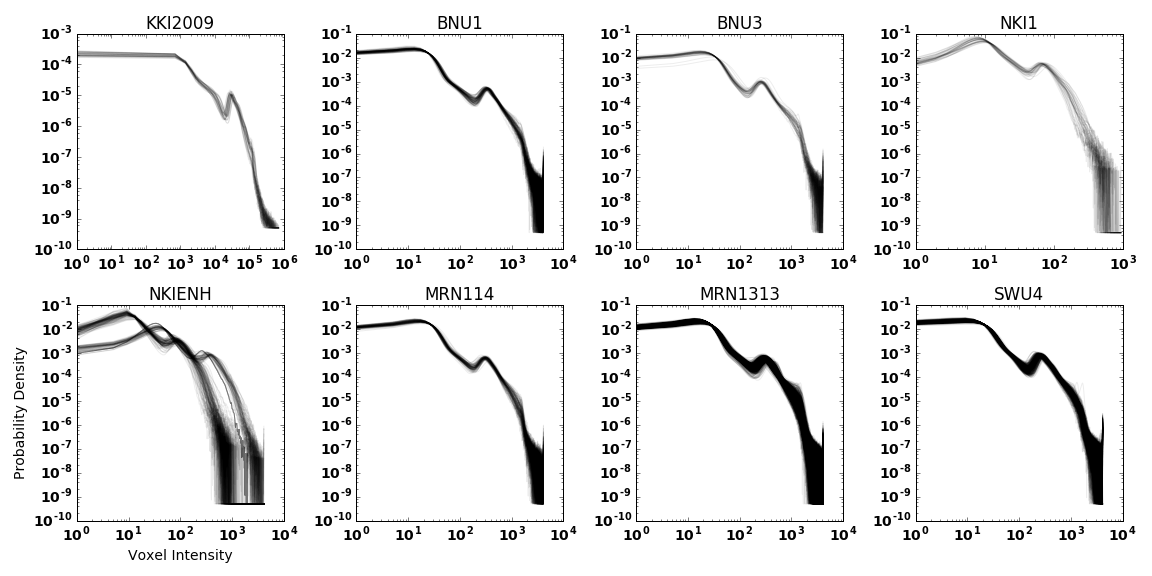
\includegraphics[width=1\textwidth]{./stats/batcheffects.png}
\makeatletter
\let\@currsize\normalsize
\caption{Histograms of B0 volumes for various datasets. The darkness of the line indicates the number of overlapping scan histograms.}
\label{fig:b0s}
\end{figure}

\subsection{Graphs}
All selected metrics were computed on several datasets, including KKI2009, MRN114, and SWU4, all parcellated to the Desikan 70 node atlas. One set of figures is explored here while others can be found in Appendix \ref{app:graphs}. Here we explore the results of the KKI2009 dataset.

\begin{figure}[h!]
\centering
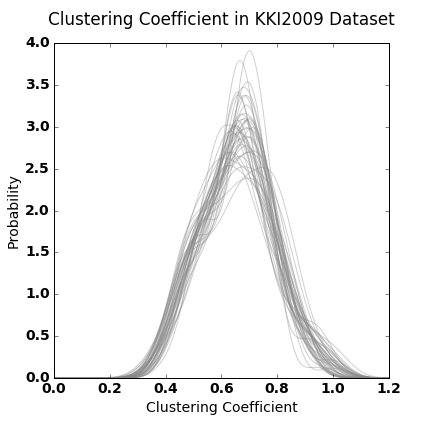
\includegraphics[width=0.4\textwidth]{./stats/KKI2009-cc.png}
\makeatletter
\let\@currsize\normalsize
\caption{Clustering coefficients for KKI2009 dataset.}
\end{figure}

The first metric analyzed was the clustering coefficient. Colloquially, the clustering coefficient is the degree to which the nodes group together or cluster, naturally. In the KKI2009 dataset, the mode in most graphs lies around a coefficient of 0.7. The MRN114 dataset contains several outliers, with the dominant mode being 0.8, and the SWU4 dataset similarly to MRN114 contains several outlier graphs, with a mode of 0.8.

The number of non-zero edges in a dataset provides an indication of how sparse the graphs are. In this case, the Desikan atlas contains 70 nodes. This means that there are a total possible 2415 unique edges.
\begin{figure}[h!]
\centering
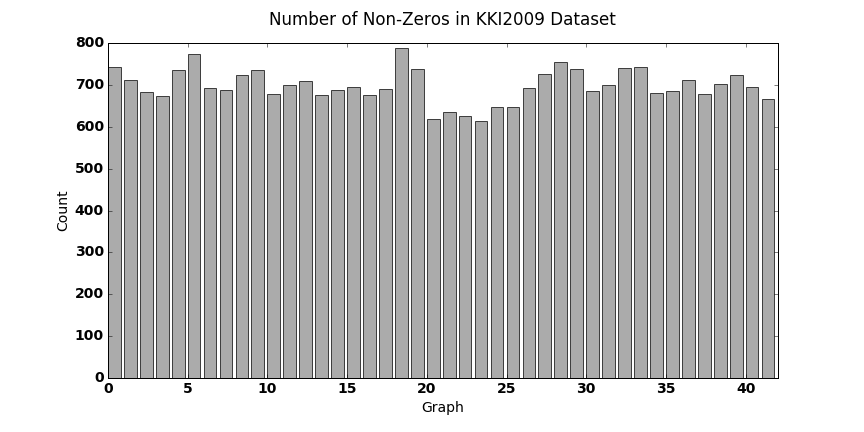
\includegraphics[width=0.8\textwidth]{./stats/KKI2009-nnz.png}
\makeatletter
\let\@currsize\normalsize
\caption{Number of non-zero edges for KKI2009 dataset.}
\end{figure}
In the KKI2009 dataset, we see that the average number of non-zero edge weights is approximately 700, with relatively low variance. In both the MRN114 and SWU4 datasets, however, we have much higher variance and a mean of approximately 1300 non-zero edges. This means that, edge weights aside, the KKI2009 graphs are considerably more sparse than these other two datasets.

The betweenness centrality of nodes in the graph indicate the centrality of that node to the graph as a whole. This measure is a count of the number of shortest paths between nodes that passes through the node of interest. We can see in the KKI2009 dataset that the distribution of the betweenness centrality is very heavily left-shifted, indicating that there are not many clearly central nodes in the graphs. The MRN114 and SWU4 datasets are similar to KKI2009, though even shifted closer towards 0.
\begin{figure}[h!]
\centering
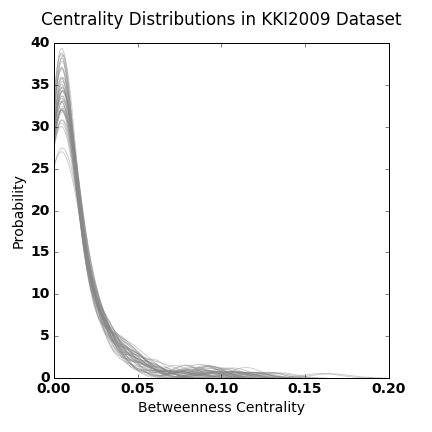
\includegraphics[width=0.4\textwidth]{./stats/KKI2009-centrality.png}
\makeatletter
\let\@currsize\normalsize
\caption{Betweenness centrality for KKI2009 dataset.}
\end{figure}

The degree of a node is simply a count of the number of adjacent nodes via edges (unweighted) to the node in question. The KKI2009 dataset is very consistent, with most graphs having a mode degree of 20.
\begin{figure}[h!]
\centering
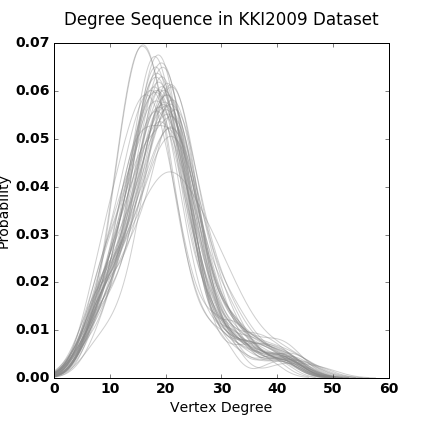
\includegraphics[width=0.4\textwidth]{./stats/KKI2009-degree.png}
\makeatletter
\let\@currsize\normalsize
\caption{Degree sequence for KKI2009 dataset.}
\end{figure}
Similarly to all of the previous metrics, the SWU4 and MRN114 datasets contain much more variance, with a mode that is higher, at approximately 40.
The edge weights in graphs produced by ndmg, as described previously, are determined by the number of fibers connecting the two regions of interest in our parcellation. This means that in larger parcellations, the edge weights will naturally be lower, as fewer voxels in the image are aggregated into each node in the graph. As expected, many of the edges are of low weight, as single or few fibers pass between regions. However, the distributions seen here have a fairly wide tail and contain considerable density in edge weights up to 10,000 fibers in the KKI2009 dataset. Similarly, these tails extend in the MRN114 and SWU4 datasets to 20,000 fibers approximately.
\begin{figure}[h!]
\centering
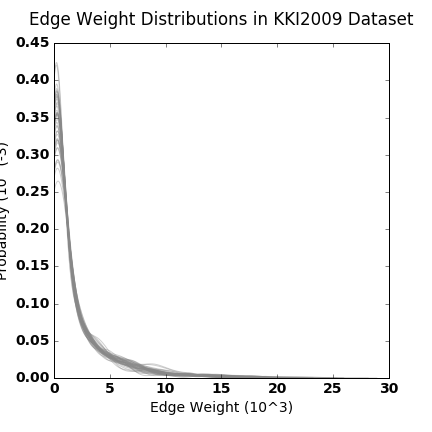
\includegraphics[width=0.4\textwidth]{./stats/KKI2009-edgeweight.png}
\makeatletter
\let\@currsize\normalsize
\caption{Edge weight distributions for KKI2009 dataset.}
\end{figure}

\section{Web services}
\label{sec:webservices}
In order increase accessibility of our tool and data even further, several web services have been created to both share existing data and process connectomes from new data. The back-end of the web services have been engineered by Disa Mhembere, while the processing algorithms were primarily a result of my work.

\subsection{MR-GRUTEDB}
\label{sec:mrgrutedb}
All of the data processed by ndmg has been pushed to our graph database, \textsc{mr-grutedb} (MR Graph with Rich atribUTE DataBase). The database can be accessed through our website, \url{http://openconnecto.me/graph-services/download/}, and provides easy access to large volumes of data. This database enables users to query graphs based on their number of nodes, edges, the dataset which they belong to, and what attributes exist in the graph. This database and web service has been built using Django, and a RESTful endpoint exists so that a user may programmatically access the database and interact with it as if they were on the website purely from code, if they wish to streamline their analyses.

\subsection{C4}
\label{c4}
Also built using the Django web framework, the C4 web service (Community Connectomics via Cloud Computing) allows users to upload MR images, and in a single click receive a connectome in return. Accessible through \url{http://openconnecto.me/graph-services/c4/}, users can also download sample data in order to test our pipeline quickly. The web server hosting this service runs on a machine that is connected to a submission queue for a high performance computing node. When files are uploaded by a user, they are transferred to this server and a job is submitted to the queue, as well as an email to the user letting them know that the service has accepted their files. The ndmg pipeline takes approximately 30-60 minutes to compute a connectome from DTI data with ~40-110 diffusion directions, respectively. Upon job completion, the produced graph and other derivatives are stored publicly on \url{http://openconnecto.me/mrdata/c4/}, and an email sent to the user indicating their specific data location. This service is free of charge, and open to the public. Currently, the service only enables single subjects to be processed per submission, but users with datasets consisting of many subjects are able to contact us and we will process their data for them. All data processed through this service must be de-identified in a HIPPA compliant fashion prior to uploading, as our service has not been developed to handle confidential data and all derivatives are stored publicly.
%=========================
%%% End Results


%%% Begin Conclusion
%=========================
\chapter{Conclusion}
Connectomics is a young discipline which shows promise for understanding both the structure and function of the brain. However, being such a young field means that the availability of tools, services, and data to aid in connectomics research is limited. We have designed and produced a one click open source reliable pipeline which computes connectomes at multiple resolutions from MR images. We have packaged this pipeline in a web service that is free of charge, and provide a database containing connectomes generated from all known publicly available and redistributable MRI datasets containing both T1 and DTI.

%=========================
%%% End Conclusion